\documentclass[12pt,a4paper,twoside,openright]{report}

% BASIC SETTINGS
\usepackage{moreverb}								% List settings
\usepackage{textcomp}								% Fonts, symbols etc.
\usepackage{lmodern}								% Latin modern font
\usepackage{helvet}									% Enables font switching
\usepackage[T1]{fontenc}							% Output settings
\usepackage[english]{babel}							% Language settings
\usepackage[utf8]{inputenc}							% Input settings
\usepackage{amsmath}								% Mathematical expressions (American mathematical society)
% \usepackage{amssymb}								% Mathematical symbols (American mathematical society)
\usepackage{graphicx}								% Figures
% \usepackage{subfig}									% Enables subfigures
\numberwithin{equation}{chapter}					% Numbering order for equations
\numberwithin{figure}{chapter}						% Numbering order for figures
\numberwithin{table}{chapter}						% Numbering order for tables
\usepackage{minted}						    		% Enables source code listings
% \usepackage{chemfig}								% Chemical structures
\usepackage[top=3cm, bottom=3cm,
			inner=3cm, outer=3cm]{geometry}			% Page margin lengths
\usepackage{eso-pic}								% Create cover page background
\newcommand{\backgroundpic}[3]{
	\put(#1,#2){
	\parbox[b][\paperheight]{\paperwidth}{
	\centering
	\includegraphics[width=\paperwidth,height=\paperheight,keepaspectratio]{#3}}}}
\usepackage{float} 									% Enables object position enforcement using [H]
\usepackage{parskip}								% Enables vertical spaces correctly


\usepackage[utf8]{inputenc}
\usepackage[english]{babel}
\usepackage{csquotes}
\usepackage{hyperref} % For hyperlinks in the PDF
\usepackage{url}
\usepackage{amsfonts}
\usepackage{tikz}
\usepackage{subcaption}

\usepackage{footnote}
\makesavenoteenv{tabular} % For footnotes inside tabular
\makesavenoteenv{table}

\usepackage[toc,page]{appendix}

%\usepackage[backend=biber]{biblatex}
\usepackage[style=authoryear-comp,
            urldate=iso8601,
            maxbibnames=99,
            maxcitenames=3,
            backend=biber]{biblatex}


% OPTIONAL SETTINGS (DELETE OR COMMENT TO SUPRESS)

% Disable automatic indentation (equal to using \noindent)
\setlength{\parindent}{0cm}


% Caption settings (aligned left with bold name)
\usepackage[labelfont=bf, textfont=normal,
			justification=justified,
			singlelinecheck=false]{caption}


% Activate clickable links in table of contents
\usepackage{hyperref}
\hypersetup{colorlinks, citecolor=black,
   		 	filecolor=black, linkcolor=black,
    		urlcolor=black}


% Define the number of section levels to be included in the t.o.c. and numbered	(3 is default)
\setcounter{tocdepth}{5}
\setcounter{secnumdepth}{5}


% Chapter title settings
\usepackage{titlesec}
\titleformat{\chapter}[display]
  {\Huge\bfseries\filcenter}
  {{\fontsize{50pt}{1em}\vspace{-4.2ex}\selectfont \textnormal{\thechapter}}}{1ex}{}[]


% Header and footer settings (Select TWOSIDE or ONESIDE layout below)
\usepackage{fancyhdr}
\pagestyle{fancy}
\renewcommand{\chaptermark}[1]{\markboth{\thechapter.\space#1}{}}


% Select one-sided (1) or two-sided (2) page numbering
\def\layout{2}	% Choose 1 for one-sided or 2 for two-sided layout
% Conditional expression based on the layout choice
\ifnum\layout=2	% Two-sided
    \fancyhf{}
	\fancyhead[LE,RO]{\nouppercase{ \leftmark}}
	\fancyfoot[LE,RO]{\thepage}
	\fancypagestyle{plain}{			% Redefine the plain page style
	\fancyhf{}
	\renewcommand{\headrulewidth}{0pt}
	\fancyfoot[LE,RO]{\thepage}}
\else			% One-sided
  	\fancyhf{}
	\fancyhead[C]{\nouppercase{ \leftmark}}
	\fancyfoot[C]{\thepage}
\fi


% Enable To-do notes
\usepackage[textsize=tiny]{todonotes}   % Include the option "disable" to hide all notes
\setlength{\marginparwidth}{2.5cm}


% Supress warning from Texmaker about headheight
\setlength{\headheight}{15pt}



% http://tex.stackexchange.com/questions/285578/how-to-draw-parallelepiped-and-cube-with-latex
\usetikzlibrary{quotes,arrows.meta,arrows}
\tikzset{
  annotated cuboid/.pic={
    \tikzset{%
      every edge quotes/.append style={midway, auto},
      /cuboid/.cd,
      #1
    }
    \draw [every edge/.append style={pic actions, densely dashed, opacity=.5}, pic actions]
    (0,0,0) coordinate (o) -- ++(-\cubescale*\cubex,0,0) coordinate (a) -- ++(0,-\cubescale*\cubey,0) coordinate (b) edge coordinate [pos=1] (g) ++(0,0,-\cubescale*\cubez)  -- ++(\cubescale*\cubex,0,0) coordinate (c) -- cycle
    (o) -- ++(0,0,-\cubescale*\cubez) coordinate (d) -- ++(0,-\cubescale*\cubey,0) coordinate (e) edge (g) -- (c) -- cycle
    (o) -- (a) -- ++(0,0,-\cubescale*\cubez) coordinate (f) edge (g) -- (d) -- cycle;
    \path [every edge/.append style={pic actions, |-|}]
    (b) +(0,-5pt) coordinate (b1) edge ["\cubex \cubeunits"'] (b1 -| c)
    % (b) +(-5pt,0) coordinate (b2) edge ["\cubey \cubeunits"] (b2 |- a)
    % (c) +(3.5pt,-3.5pt) coordinate (c2) edge ["\cubez \cubeunits"'] ([xshift=3.5pt,yshift=-3.5pt]e)
    ;
  },
  /cuboid/.search also={/tikz},
  /cuboid/.cd,
  width/.store in=\cubex,
  height/.store in=\cubey,
  depth/.store in=\cubez,
  units/.store in=\cubeunits,
  scale/.store in=\cubescale,
  width=10,
  height=10,
  depth=10,
  units=,
  scale=.005,
}

\renewcommand{\cite}{\parencite}




\addbibresource{bibs/classic_htr.bib}
\addbibresource{bibs/deep_learning.bib}
\addbibresource{bibs/digit_recognition.bib}
\addbibresource{bibs/familysearch.bib}
\addbibresource{bibs/references.bib}

% \graphicspath{ {pictures/} }


% \author{\normalsize Leif Schelin \\
% 	\normalsize 911016-3574 \\
% 	\normalsize scleif@student.chalmers.se}
%\date{November 2016}

\begin{document}
% \tracingall

% \maketitle

% \vspace{4cm}

\newpage

%------------------------------

% TODO: perhaps make a Glossary? HTR, CNN, indexing etc.

\pagenumbering{roman}


% COVER PAGE
\begin{titlepage}
\newgeometry{top=3cm, bottom=3cm,
			left=2.25 cm, right=2.25cm}	% Temporarily change margins		
			
% Cover page background 
\AddToShipoutPicture*{\backgroundpic{-4}{56.7}{figures/auxiliary/frontpage_gu_eng.pdf}}
\addtolength{\voffset}{2cm}

% Cover picture (replace with your own or delete)	

% \begin{figure}[H]
% \centering
% \vspace{1cm}	% Adjust vertical spacing here
% \includegraphics[width=0.9\linewidth]{figure/Wind.png}
% \end{figure}

% Cover text
\mbox{}
\vfill
\renewcommand{\familydefault}{\sfdefault} \normalfont % Set cover page font
\textbf{{\Huge 	
Classification of Handwritten Historical \\[0.2cm]
Documents with Visual Attention
% Classification of Handwritten Historical Documents: %\\[0.2cm]
% Convolutional Neural Networks and Visual Attention
% Waypointing of Historical Documents by Deep Learning%   \\[0.2cm] 
				% Master's thesis template for \LaTeX
				}} 	\\[0.5cm]
% {\Large A Subtitle that can be Very Much Longer if Necessary}\\[0.5cm]
Master's thesis in Computer Science -- algorithms, language and logic \setlength{\parskip}{1cm}

{\Large LEIF SCHELIN} \setlength{\parskip}{2.9cm}

Department of Computer Science and Engineering \\
\textsc{Chalmers University of Technology} \\
\textsc{University of Gothenburg} \\
Gothenburg, Sweden 2017

\renewcommand{\familydefault}{\rmdefault} \normalfont % Reset standard font
\end{titlepage}


% BACK OF COVER PAGE (BLANK PAGE)
\newpage
\restoregeometry
\thispagestyle{empty}
\mbox{}


% TITLE PAGE
\newpage
\thispagestyle{empty}
\begin{center}
	\textsc{\large Master's thesis 2017}\\[4cm]		% Report number is currently not in use
	\textbf{\Large 
	Classification of Handwritten Historical  \\[0.2cm]
	Documents with Visual Attention
	%: \\
%Convolutional Neural Networks and 
% 	Waypointing of Historical Documents by Deep Learning
	%\\ the Content of the Report
	} \\[1cm]
% 	{\large A Subtitle that can be Very Much Longer if Necessary}\\[1cm]
	{\large LEIF SCHELIN}
	
	\vfill	
	% Logotype on titlepage	
	\begin{figure}[H]
	\centering
	% Remove the following line to remove the titlepage logotype
	
\includegraphics[width=0.4\pdfpagewidth]{figures/auxiliary/logo_ch_gu.pdf}
	%
\includegraphics[width=0.2\pdfpagewidth]{figure/auxiliary/logo_eng.pdf}
	\end{figure}	\vspace{5mm}	
	
	Department of Computer Science and Engineering\\
	%\emph{Division of Division name}\\
	%Name of research group (if applicable)\\
	\textsc{Chalmers University of Technology} \\
	\textsc{University of Gothenburg} \\
	Gothenburg, Sweden 2017 \\
\end{center}


% IMPRINT PAGE (BACK OF TITLE PAGE)
\newpage
\thispagestyle{plain}
\vspace*{4.5cm}
Classification of Handwritten Historical Documents with Visual Attention \\
% Classification of Handwritten Historical Documents: \\
% Convolutional Neural Networks and Visual Attention \\
% Waypointing of Historical Documents by Deep Learning\\
% A Subtitle that can be Very Much Longer if Necessary\\
LEIF SCHELIN \setlength{\parskip}{1cm}

\copyright ~ LEIF SCHELIN, 2017. \setlength{\parskip}{1cm}

Supervisor: Rebecka Jörnsten, Division of Applied Mathematics and Statistics\\
Advisor: Jon Morrey and Randy Wilson, FamilySearch\\
Examiner: Peter Damaschke, Department of Computer Science and Engineering \setlength{\parskip}{1cm}

Master's Thesis 2017\\	% Report number currently not in use 
Department of Computer Science and Engineering\\
%Division of Division name\\
%Name of research group (if applicable)\\
Chalmers University of Technology
and University of Gothenburg\\
SE-412 96 Gothenburg\\
Telephone +46 31 772 1000 \setlength{\parskip}{0.5cm}

\vfill
% Caption for cover page figure if used, possibly with reference to further information in the report

% Cover: Wind visualization constructed in Matlab showing a surface of constant wind speed along with streamlines of the flow. \setlength{\parskip}{0.5cm}

Typeset in \LaTeX \\
%Printed by [Name of printing company]\\
Gothenburg, Sweden 2017



\setlength{\parindent}{0em}
\setlength{\parskip}{0em}

\newpage
Classification of Handwritten Historical Documents with Visual Attention \\
% Classification of Handwritten Historical Documents: \\
% Convolutional Neural Networks and Visual Attention \\
% Waypointing of Historical Documents by Deep Learning\\
% A Subtitle that can be Very Much Longer if Necessary\\
LEIF SCHELIN\\
Department of Computer Science and Engineering\\
Chalmers University of Technology and University of Gothenburg\setlength{\parskip}{0.5cm}

\thispagestyle{plain}			% Supress header
% \setlength{\parskip}{0pt plus 1.0pt}
\section*{Abstract}

We introduce a new dataset for extracting genealogical information consisting of Swedish population records and weak labels.
Inspired by recent progress in deep learning and computer vision, we suggest and evaluate an end-to-end trainable deep learning model based on convolutional neural networks as well as several loss functions for extracting the year from each page.
We show how our model partially recognizes year from locating and transcribing the written year and partially from recognizing typical handwriting styles.
Finally we provide a baseline on this dataset and suggest future work for automatically extracting genealogical information from population records.

% KEYWORDS (MAXIMUM 10 WORDS)
\vfill
Keywords: Deep learning, convolutional neural networks, attention models, handwriting recognition, information extraction, genealogy.

\newpage				% Create empty back of side
\thispagestyle{empty}
\mbox{}


\newpage
\thispagestyle{plain} % Supress header
\section*{Acknowledgements}

I send my gratitude and regards to my supervisor Rebecka Jörnsten, whose enthusiasm and ideas have greatly benefited the project.

I also thank Jon Morrey and Randy Wilson from FamilySearch, without whose data this thesis would not have been possible.

Lastly, I want to thank my wife Mai for her considerate loving support from the idea stage to the conclusion of the thesis.

\vspace{1.5cm}
\hfill
% TODO: check/update date
Leif Schelin, Gothenburg, May 2017

\newpage
\thispagestyle{empty}
\mbox{}


% \newpage
% 
\section*{Preface}
\textbf{TODO...}


\newpage
\tableofcontents
\addcontentsline{toc}{chapter}{\contentsname}

% List of figures (add to table of contents)
\cleardoublepage
\listoffigures
\addcontentsline{toc}{chapter}{\listfigurename}

% List of tables (add to table of contents)
\cleardoublepage
\listoftables
\addcontentsline{toc}{chapter}{\listtablename}


\cleardoublepage
\setcounter{page}{1}
\pagenumbering{arabic}			% Arabic numbering starting from 1 (one)
% \setlength{\parskip}{0pt plus 1pt}

\setlength{\parskip}{0.5em}
\setlength{\parindent}{1em}

% Motivation for the thesis

\chapter{Introduction}

FamilySearch is a large non-profit genealogy organization \cite{FamilySearchAbout}. They have been photographing handwritten historical population records in many countries for many years.

In 2006, the \textbf{Indexing} project started where volunteers manually extract relevant information from the photographed pages \cite{Indexing}. The extracted (\textbf{indexed}) information is quality-checked and then published on the organization's website FamilySearch.org where users can search for information about their ancestors.
In 2013, over 1 billion data posts for births, deaths and marriages had been indexed by volunteers \cite{Billion}.

The number of photographed pages grow faster than what the available pool of volunteers can process. Thus, there is a need for automating as much of the indexing work as possible. However, indexing is difficult to automate because (1) the records are written in different languages, (2) they come from a vast array of locations and periods in time and (3) there is considerable variation in both spelling and page structure.
The handwriting style differs from scribe to scribe although it may be somewhat similar during the same time period in the same region.
%Although the handwriting style may be similar during the same time period, individual scribes write differently.
% there is considerable variance between different scribes.

If the images were correctly transcribed by a \textbf{handwritten text recognition} (HTR) system, it would still take considerable natural language processing to extract the information, especially since there is little training data for languages over different time periods.

An easier problem to solve than extracting all relevant information in the images is grouping the images by year, record type and location. This task is called \textbf{waypointing} \cite{Waypointing} and it currently requires considerable manual labor by genealogy experts.

Annotating each image with year, record type and location would solve waypointing as well as constitute a stepping stone towards fully or partially automated indexing.
Image annotation is an easier problem than handwriting recognition because it only needs to consider information which belongs to a small domain compared to the full vocabulary of a natural language and all possible names.


\section{Genealogy}

Genealogy is the study of one's ancestors. It involves finding who they were, the time and place of their births, where they lived, how their lives were, how their lives eventually ended and how their families continued to present day.

Getting to know and comprehend the lives of one's ancestors can have great personal significance as one can feel more connected with people in centuries past. It may increase the appreciation for parents and forefathers and their efforts so that oneself could be born.
Experiences can also be learned from important events, stories and hardships in the lives of one's ancestors and
%one can more easily appreciate
it becomes more apparent
how many things are different today, although as human beings we are perhaps not so different.

Many people are familiar with the lives of their parents and perhaps also the their grandparents from just listening to them.
However, each generation further back requires more study and effort to explore as the records get more sparse, get harder to access, are written in an older language and in a handwriting style that get increasingly different from the handwriting of today. Furthermore, because each child has two biological parents, the number of ancestors increases at least by a factor of two in each generation.

The advance of technology has been very instrumental in making the genealogical research easier and more accessible. Instead of traveling to different vaults of the records, people could order microfilms with photographs to view at home or at a nearby genealogy center. With the Internet, people can currently access many records directly online as images. A future big leap forward consists of the indexing effort which makes it possible for people to search the records with search engines and databases instead of manually scanning through and reading the pages.

Manually indexing a book from cover to cover has a very high throughput of data compared to searching the pages for a single entry because (1) it takes time to get accustomed to the handwriting of that particular scribe as well as locations in that parish and (2) the time for each entry is significantly reduced as one does not need to search through many pages. So, although it is not viable for a single person to do, if many people contribute, it lowers the total workload in the end for the community.

However, indexing takes a lot of effort and also some experience in reading old handwriting. If computers could index the records themselves with only minor human contribution, that would significantly improve the indexing rate and hence produce a very powerful tool for the entire genealogical community.

Solving waypointing is not as significant as indexing but would constitute a stepping stone towards indexing by extracting information from the records in an automated manner.
% as well as reducing manual labor for waypointing.
Waypointing in itself is also useful as more images can be published online under the correct categories. Automating waypointing would free time in favor of genealogical research and indexing.

\section{Goals}

The goal of the thesis is to make an open-source prototype that automatically extracts high-level information for each photographed page of historical population records. The information under consideration is 1. year, 2. page number and 3. record type, where the record type is one of \{blank, birth, death, marriage\}.
% If time permits, extracting location (such as parish) will also be considered.

The system should learn from the currently indexed and waypointed data in a fully autonomous manner without explicit feature engineering.
% However, standard pre-processing techniques such as median filtering and gray level normalization may be necessary.

%A perfect classification is unrealistic so the resulting groupings of images will need some manual inspection before publication. However, it should be sufficient to check some of the pages in a group instead of going through every page. Thus the manual workload should be significantly decreased. If the precision of the system is too low, correcting errors would be equally troublesome as doing the waypointing manually. Thus, the precision of the classification should be as high as possible.

% While maximizing the precision, the system should have a reasonable throughput. Processing millions of photographed pages should be viable.

\section{Delimitation}

Although FamilySearch has indexed images in many languages from many places,
%Although there are images in many languages from many places,
the thesis only considers images of handwritten text in a single language from a single country but over a longer period of time, possibly up to three hundred years.
However, the techniques applied should be general enough to handle many different languages.
%, at least for extracting year and page number.

% We primarily consider deep learning techniques for solving the problem in contrast to conventional methods of handwriting recognition.

In order to simplify the model,
the system will classify each page with a single year although there may be none or several years present. For example, one photograph can contain baptisms from 1793 to 1797. In order to solve indexing, it is however necessary to correctly recognize all present values.


\subsection{Related work}
...



\section{Datasets}

Here we describe some existing datasets for historical handwriting recognition and information extraction. We also consider their usefulness in regard to the thesis.

% TODO add pictures for some of the datasets?


\subsection{MNIST}

The MNIST database contains $70000$ normalized images of handwritten digits \cite{MNIST_orig}. All images have the fix size $28 \times 28$ pixels. The dataset is very popular for testing new algorithms and machine learning models \cite{MNIST}.
% It is even used for the introductory tutorial of Tensorflow \cite{}.
% https://www.tensorflow.org/get_started/mnist/pros
Although we can not use MNIST to evaluate the proposed models in this thesis, the dataset is useful for quick experimentation and pre-training. We discuss this further in section \ref{ssec:pretrain}.

\subsection{Historical documents}
Several collections of historical documents have been line segmented and transcribed for public use \cite{esposalles}: George Washington, Parzival, Saint Gall, RODRIGO and GERMANA. However, they consist of prose written by one or two scribes and not civil population records which are typically written by many different scribes.
% TODO add citations for each mentioned data set?

\subsection{Esposalles}
In contrast, the Esposalles dataset consists of book indices and historical marriage licenses from the Cathedral of Barcelona \cite{esposalles}. Experts have manually segmented and transcribed each word exactly as they occur in the image.

Although the Cathedral of Barcelona holds 291 books containing approximately 600 000 marriage licenses between 1451 and 1905, only a tiny fraction of this collection has been transcribed for the Esposalles dataset. The dataset consists of 173 pages from a single book written by a single scribe, containing 1747 marriage licenses between 1617 and 1619. Additionally, the dataset contains 29 pages of book indices.

The Esposalles dataset was used as ground truth for named entity recognition in the Robust reading competition at the International Conference on Document Analysis and Recognition (ICDAR) 2017 \cite{EsposallesCompetition}. For the competition, the words have been annotated with semantic categories such as surname of husband and surname of wife.

We think that the exact transcriptions, bounding boxes and annotations make the dataset useful for segmentation-based methods in tasks like word segmentation, handwriting recognition and named entity recognition.
Specifically for this thesis, we intend to classify years in a much larger range than 1617 to 1619 so the Esposalles dataset is simply too small. Furthermore, we are interested in exploring segmentation-free methods so we would not take advantage of the bounding boxes present in this dataset.

% TODO perhaps argue about slow and expensive process?
% We argue that creating a dataset of exact transcriptions and annotations by using paleographical experts is too slow and expensive to make a sufficiently large

%Furthermore, we believe that in order to make a system for fully automated indexing, the dataset needs to cover many more examples. Since using paleographical experts to transcribe and annotate each word is a slow and expensive process we do not expect the dataset to grow quickly.
% Thus, we assume that in order to create a sufficiently large dataset for training
%Thus we argue that for a dataset to grow sufficiently large it should
%1. not require the transcriber to be an expert and 2.
%only contain the most vital coarse information instead of every single word.


\subsection{IRIS}

While the Esposalles dataset focus on individual words transcribed by experts, the IRIS dataset contain record information extracted by volunteers in FamilySearch's indexing program \cite{Iris}.
Thus the extracted information does not contain exact transcriptions of the text but rather the most important semantic contents.
For example, abbreviations may have been expanded, dittos replaced by their intended values and information that was deemed genealogically irrelevant has been ignored.
Furthermore, while in Esposalles each transcribed word has a manually created bounding box, in IRIS there is no indication about what part of the image the information was extracted from.

The IRIS dataset consist of four collections of population records, totaling nearly $50000$ images:

\paragraph{1, 2}
The first two collections in the IRIS dataset are the 1930 population census in the US and Mexico. The images consist of big tables with names and occupations in the cells.
For the purpose of this thesis where we extract the written year for each page, the 1930 censuses are not directly useful since they only contains records from a single year. Furthermore, it is not clear that if a system can learn from this collection that it would by useful for any other collection.
However because the 1930 censuses are written on printed tables, word segmentation should be considerably simpler than for the free-form writing as in other collections.

\paragraph{3}
The third collection contains marriage licenses between 1837-1944 in Arkansas. The marriage licenses are printed templates with handwritten text in the blanks.
It is likely that the system would learn to recognize the printed template and hence it would not be able to generalize to other collections that use different templates or free-form writing. If many collections were using the same template it would be useful to learn but then one might as well hard-code the positions of the blanks in the template. Thus, it is not very useful as training-data for models in this thesis.

\paragraph{4}
The last collection contains more than 10000 pages with records of baptisms, burials and marriages from French parishes between 1533-1906. Some of the pages contain printed templates but the majority seems to be free-form handwriting.
From manually inspecting these images, we conclude that many of them do not contain a written year anywhere on the page. These are problems that a future automated extraction system would need to handle, for this thesis however we settle for another dataset that seems somewhat easier.


\subsection{Swedish population records}

\begin{table}
\centering
\begin{tabular}{ l | r r r}
Name & Collection & Total images & Indexed images \\
\hline
Örebro	& 1647578	& 638873\footnote{\url{https://familysearch.org/search/collection/1647578}}	& 14330 \\
Uppsala	& 1647598	& 693757\footnote{\url{https://familysearch.org/search/collection/1647598}}	& 8869 \\
Södermanland	& 1647693	& 617735\footnote{\url{https://familysearch.org/search/collection/1647693}}	& 11827 \\
Kalmar	& 1930243	& 617325\footnote{\url{https://familysearch.org/search/collection/1930243}}	& 2081 \\
Jönköping	& 1930273	& 721027\footnote{\url{https://familysearch.org/search/collection/1930273}}	& 3637 \\
Västernorrland	& 1949331	& 273798\footnote{\url{https://familysearch.org/search/collection/1949331}}	& 2324 \\
\hline
Sum & & 3562515 & 43068
\end{tabular}
\caption{Collections of indexed Swedish records from FamilySearch.}
\label{tab:collections}
\end{table}


In cooperation with FamilySearch for making this thesis, we have been granted access to images and the corresponding extracted information from six collections of Swedish population records.
These collections contain records of baptisms, burials and marriages in six regions between 1627 and 1890, see Table \ref{tab:collections}. They are the Swedish counterpart of the French IRIS collection mentioned above.


\begin{figure}
    \centering
    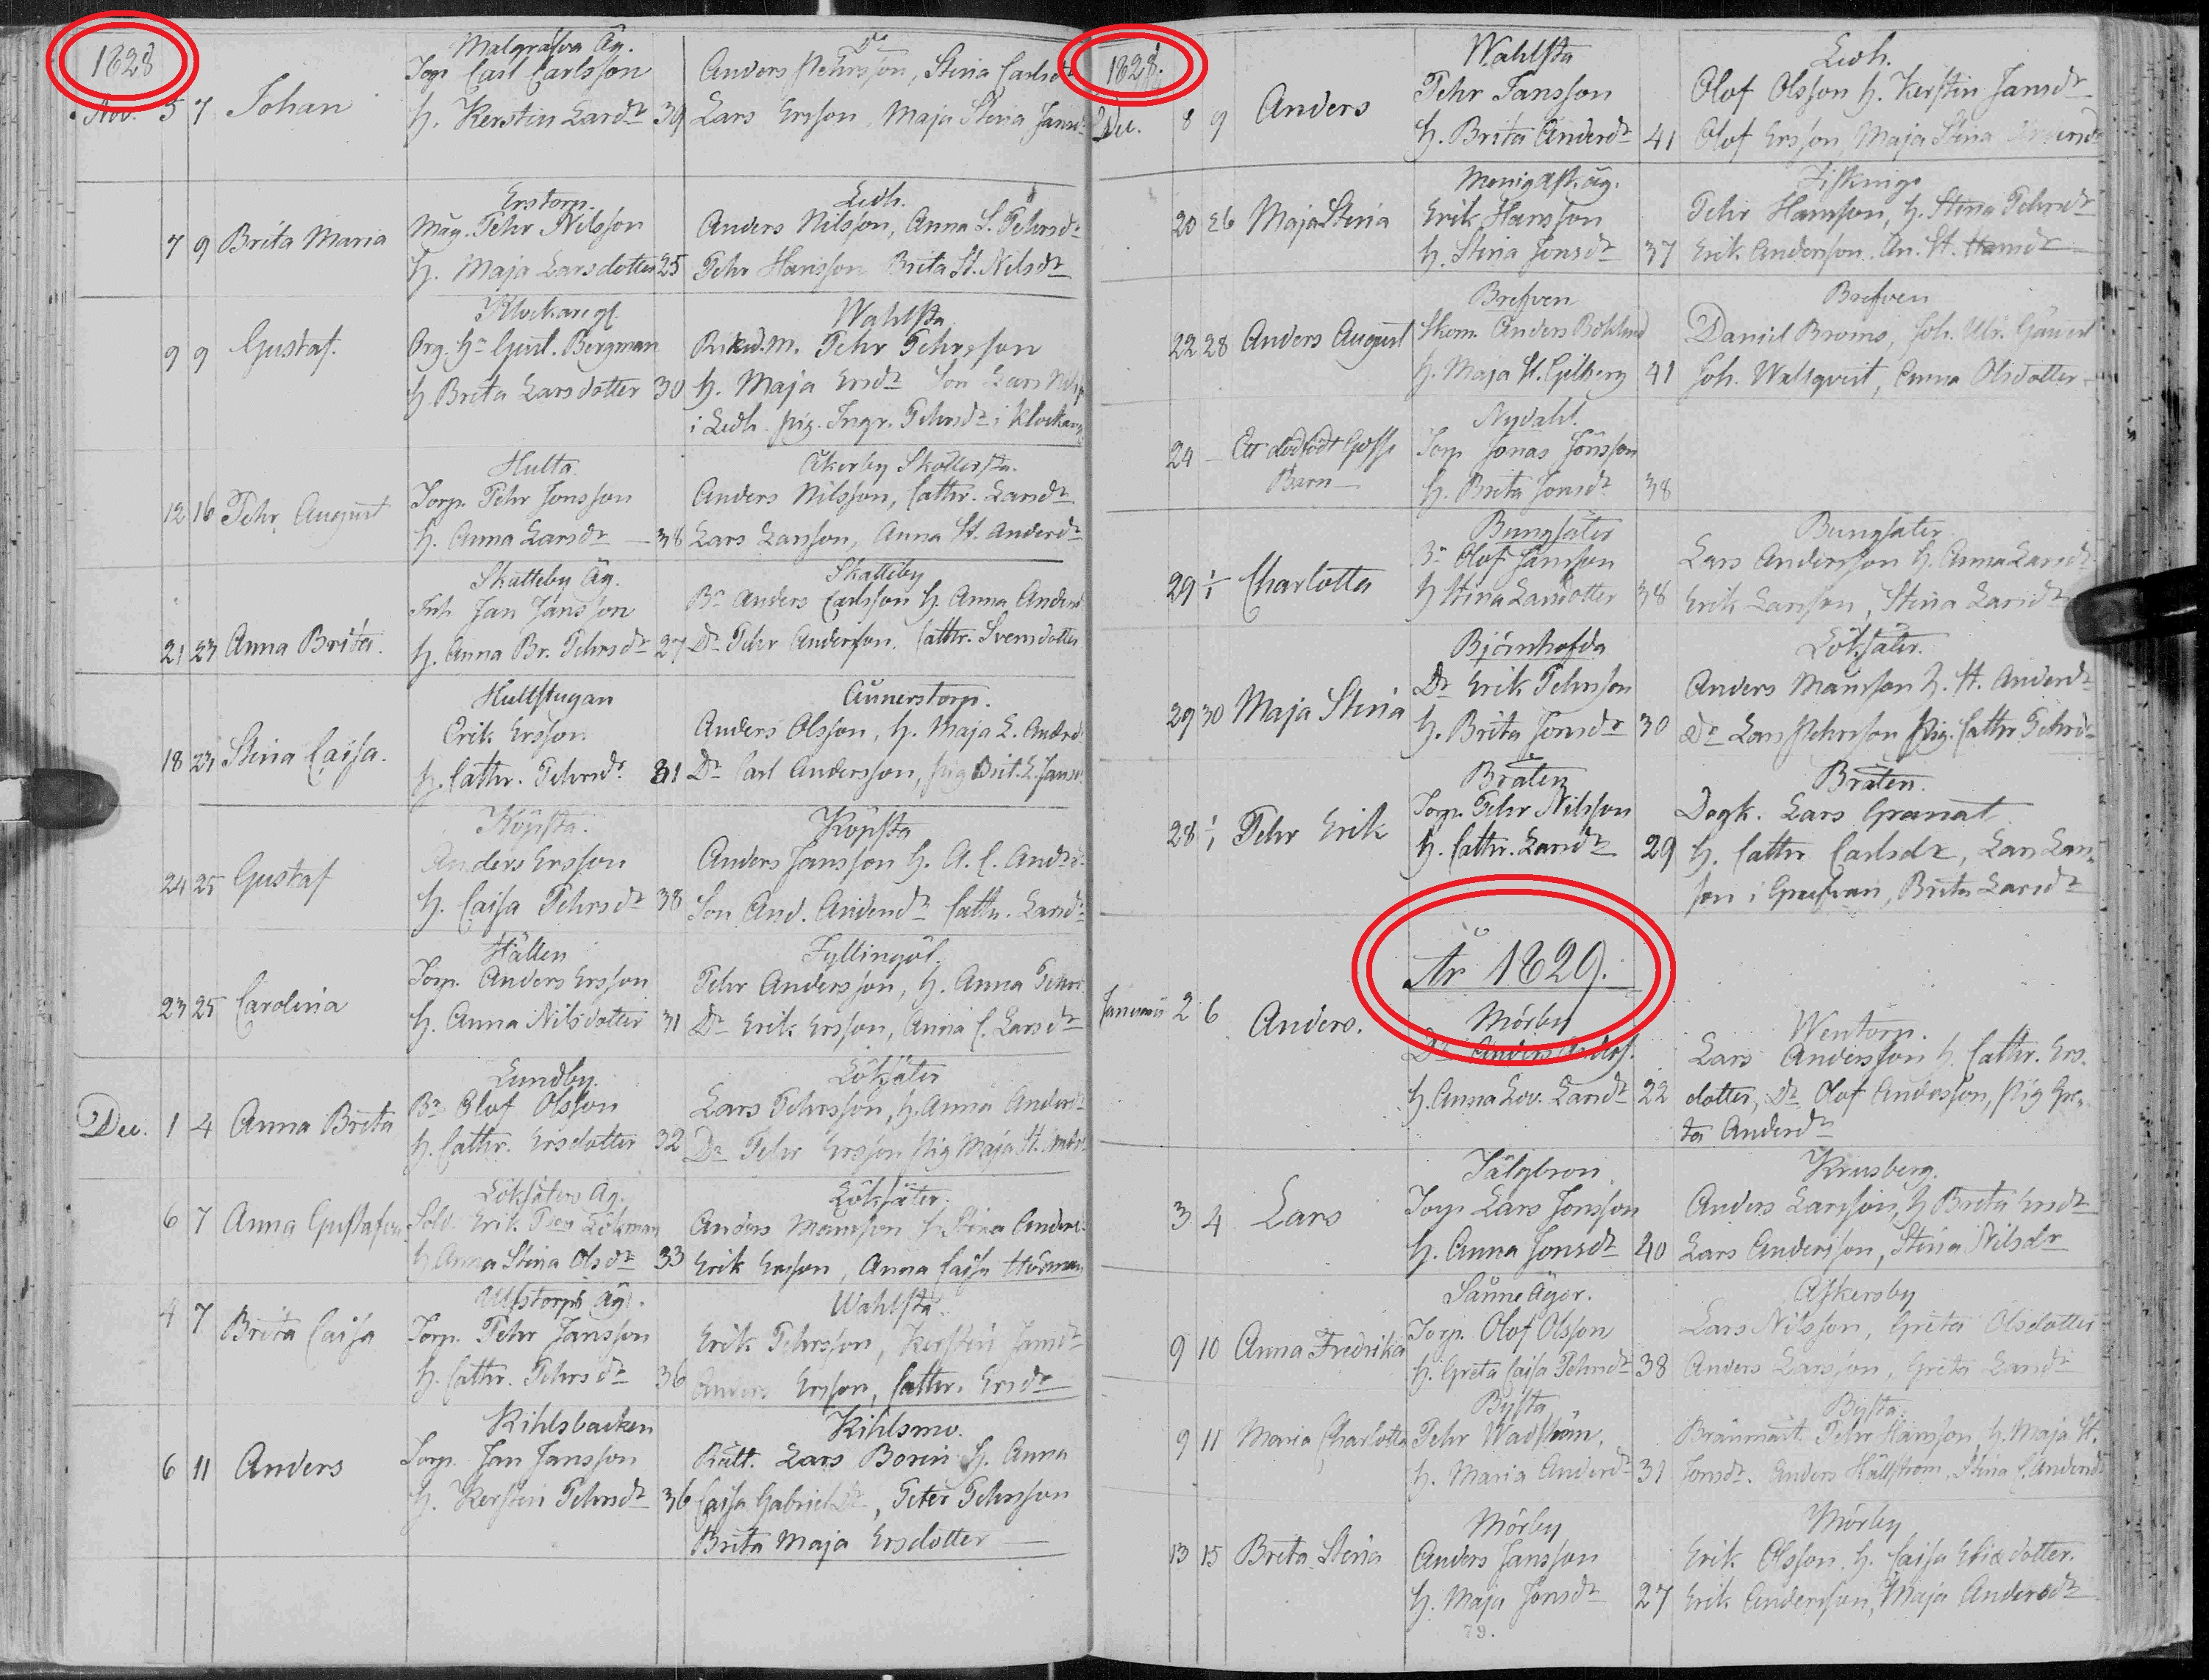
\includegraphics[scale=0.5]{resources/SWE_attention/S3HT-64P3-PQD.jpg}
    % \caption{Part of a page of burial records from the {\"O}rebro collection. Red lines have been added under the main years 1752 and 1753. There are also other years in the text such as 1687 and 1714 that we want to ignore. The picture is down-sampled to $25\%$.}
    \caption{Two pages of birth records from the book Asker C:4 in the Örebro collection. The main years, 1828 and 1829, have been emphasized with concentric ovals.}
    \label{fig:page}
\end{figure}


\subsubsection{The indexing process}

Just like with the IRIS dataset, the indexers have not provided us with bounding boxes or exact transcriptions but with extracted genealogical information. An indexed baptism record typically contains the name of the newborn child, the names of the parents, the date of birth, the date of baptism and location of the parents' home. The ecclesiastical records typically contain the names of witnesses to the baptism but this is ignored in the indexing process.

Each page is indexed by two independent volunteers. Any conflicts between the two versions is resolved by a third volunteer before submission.
The double work and review process increases the quality and consistency of the extracted information.
% Duplicating the indexing work and quality-checking increases the quality of the indexed data.
% Thus, the indexed information maintains a high quality even though it is not performed by professionals.

The extracted information is stored in the compressed GedcomX\footnote{\url{http://www.gedcomx.org/About.html}} format which has been developed specifically for genealogical information.
Each event of baptism, burial or marriage is stored as a record organized in the above mentioned six collections. Within a collection, the records do not seem to be stored in any particular order. Each record however contains information about which image it belongs to as well as some meta-information about the book the record comes from.

\subsubsection{Varying image size}

The images are stored in the JPG-format using lossy compression. Each image has a different size although the majority are about $5700 \times 4500$ pixels. There are also outliers with sizes like $7262 \times 5907$ pixels and $1885 \times 5110$ pixels. We think the varying image sizes is a result of cropping the image to fit the book in the photograph.
Since different books have different proportions, the aspect ratio of the images differs somewhat although it is often close to $1.25$:$1$.

\subsubsection{Page structure}

Each image consist of two pages. The pages are always handwritten. Sometimes the pages have pre-printed headers and vertical lines for columns, other times they are entirely free-form.
The year can often be found near the top of the page either to the left or in the middle, see Figure \ref{fig:page} for an example.


\begin{figure}
    \centering
    
\includegraphics[scale=0.3]{resources/ar_kalmar/ar1824.png}
    
\includegraphics[scale=0.3]{resources/ar_kalmar/ar1837.png}
    
\includegraphics[scale=0.3]{resources/ar_kalmar/ar1858.png}
    \caption{Three variations of the word \textquote{\r{a}r} in page headers in the Kalmar collection.}
    \label{fig:aar}
\end{figure}


Although the general structure is the same for all six collections, the exact page layout differs greatly both within and between collections. Another difference relevant for the neural network is that sometimes the year is following the word "\r{A}r" although the handwriting style for the word can be very different depending on time and place, see figure \ref{fig:aar} for some examples.


\subsubsection{Multiple years per page}

 % Additionally, when the year changed the scribe often indicated so by writing the new year in big letters before the block of new records.
Typically, the scribes did not use a new page for every new year but indicated the change of year by writing the new year in big letters before continuing to write the new records; an example of this can be seen in Figure \ref{fig:page}.
Thus besides at the top, written years can be found in virtually any part of the page. Another consequence is that a page can contain several years in a sequence like $1771, 1772, 1773, 1774$. This is especially true for small parishes where there may not have been so many burials per year. Out of the $43068$ indexed images, $16074$ or $37.3\%$ have more than one year in the extracted information.

Some images however do not contain a written year, the year is simply implied from previous pages. For such instances, indexers are instructed to search the previous and following image for an indication of the year. If the implied year is found, it is noted in the extracted information, otherwise it is indicated as unknown.
If the year is unknown or the image is blank, we ignore the image because we do not have a label for it and we expect that the year is anyway not indicated in the image. Of the indexed images, $471$ or $1\%$ have no year label.

However, in the extracted information there is no way to distinguish whether the extracted year came from the same image or if it was implied from a neighboring image. Thus, it is inevitable that some images in the dataset have labels although the year is actually not written in the image. One way to counter this problem would be to only train on images that are labeled with more than one year, expecting an indicated year change somewhere in the image. Doing so would however reduce the dataset to $37.3\%$.
Although we have no way to calculate how often the label implies a year that is missing from the image without manually inspecting every image, we assume that it is relatively rare and thus negligible.


% Provide some background on neural networks

\chapter{Neural networks}
\label{sec:networks}
\textit{
In this chapter, we first give an introduction to neural networks and deep learning in the context of classification. We then describe convolutional neural networks and their application to real tasks in computer vision, in particular for digit recognition. At the end of the chapter we summarize some recent research on deep learning for computer vision that is not used in the thesis.
For further reading about neural networks and applied deep learning to various fields, we recommend the textbook by \textcite{GoodfellowBook}.
% For a more exhaustive reading of neural networks and deep learning we recommend the reader to search out a textbook in the field such as \cite{GoodfellowBook}.
}

\section{Introduction to neural networks}

Neural networks have recently gained popularity in various fields.
% They have been observed to be quite flexible in being able to classify data, find clusters and
% Neural networks can find meaningful information in a sea of data by clustering,
Applications include finding principal components, organizing meaningful clusters in a sea of data and generating new information, for example by translating natural languages \cite{machine_translation_attention}. Here, we will focus on the task of \textbf{classification}, which refers to choosing the correct class $y$ for some given input $\mathbf{x}$. For example to correctly recognize objects in an image or to select a strategic action to take in a game.

\subsection{Multilayer perceptron}

\begin{figure}
\centering
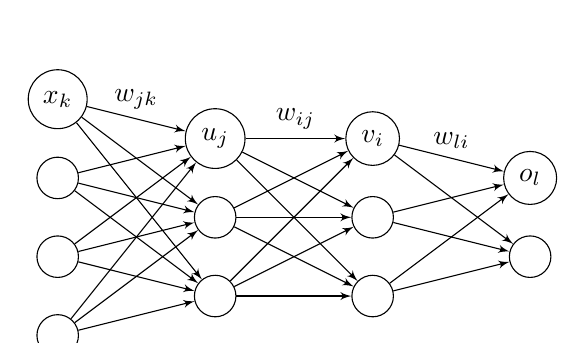
\begin{tikzpicture}

\tikzset{vertex/.style = {shape=circle,draw,minimum size=1.5em}}
\tikzset{edge/.style = {->,> = latex'}}

\node[vertex] (x1) at (0,0) {};
\node[vertex] (x2) at (0,1) {};
\node[vertex] (x3) at (0,2) {};
\node[vertex] (x4) at (0,3) {$x_k$};

\node[vertex] (v1) at (2,0.5) {};
\node[vertex] (v2) at (2,1.5) {};
\node[vertex] (v3) at (2,2.5) {$u_j$};

\node[vertex] (y1) at (4,0.5) {};
\node[vertex] (y2) at (4,1.5) {};
\node[vertex] (y3) at (4,2.5) {$v_i$};

\node[vertex] (o1) at (6,1) {};
\node[vertex] (o2) at (6,2) {$o_l$};

%edges
\draw[edge] (x1) to (v3);
\draw[edge] (x2) to (v3);
\draw[edge] (x3) to (v3);
\draw[edge] (x4) to (v3);

\draw[edge] (x1) to (v2);
\draw[edge] (x2) to (v2);
\draw[edge] (x3) to (v2);
\draw[edge] (x4) to (v2);

\draw[edge] (x1) to (v1);
\draw[edge] (x2) to (v1);
\draw[edge] (x3) to (v1);
\draw[edge] (x4) to (v1);

\draw[edge] (v1) to (y1);
\draw[edge] (v2) to (y1);
\draw[edge] (v3) to (y1);

\draw[edge] (v1) to (y2);
\draw[edge] (v2) to (y2);
\draw[edge] (v3) to (y2);

\draw[edge] (v1) to (y3);
\draw[edge] (v2) to (y3);
\draw[edge] (v3) to (y3);

\draw[edge] (y1) to (o1);
\draw[edge] (y2) to (o1);
\draw[edge] (y3) to (o1);

\draw[edge] (y1) to (o2);
\draw[edge] (y2) to (o2);
\draw[edge] (y3) to (o2);

\path[edge] (x4) -- node[above] {$w_{jk}$} (v3);
\path[edge] (v3) -- node[above] {$w_{ij}$} (y3);
\path[edge] (y3) -- node[above] {$w_{li}$} (o2);

\end{tikzpicture}

\caption{A multilayer perceptron with an input layer $x$, two hidden layers $u$ and $v$ as well as a readout layer $o$. Every connection uses a different weight $w$.}
\label{fig:mlp}
\end{figure}


A \textbf{multilayer perceptron} (MLP) is organized in several \textbf{layers}, see illustration in figure \ref{fig:mlp}. Each layer consists of a number of \textbf{neurons}.
%, the first layer has the same number as elements in the input vector $\mathbf{x}$.
Each element in the input vector $\mathbf{x}$ becomes a neuron in the \textbf{input layer}. Each neuron $v_i$ in the following layers gets its value by computing a weighted sum over the neurons $u_j$ in the previous layer using weights  $w_{ij}$, a bias term $b_i$ and an \textbf{activation function} $g$:
\[
v_i = g\left( b_i + \sum_j w_{ij} u_j \right)
\]

In order for the network to utilize the power of several layers, the activation function must be non-linear. If $g$ would be linear, then the entire network would be a series of linear transformations which could be rewritten as a single linear transformation. Traditional choices of $g$ include the hyperbolic tangent and the logistic function (which is sometimes referred to as the sigmoid function).

The final layer is called the \textbf{readout layer} and has as many neurons as there are classes. The input $\mathbf{x}$ is classified as the class $y$ which has the greatest value in the readout layer. In order to estimate the certainty, we can compute pseudo-probabilities $p_i$ of the classes by taking the \textbf{softmax} of the readout values $o_i$:
\[
p_i = \frac{ \exp(o_i) }{ \sum_k \exp(o_k) }
\]

The layers between the input layer and the readout layer are referred to as \textbf{hidden layers}.

\subsection{Backpropagation} \label{sssec:BackProp}

In order to correctly classify new input, we need to \textbf{train} the network on some existing dataset $D$ which consists of pairs of correct classifications $(\mathbf{x}^{(\mu)}, y^{(\mu)}$).
We let $\mathbf{y}^{(\mu)}$ denote a \textbf{one-hot} vector, that is all elements are zero except the indicated class whose associated element has the value one.
We then introduce a loss function $L$ to measure how different one network prediction $\mathbf{p}^{(\mu)}={\ldots, p_i^{(\mu)}, \ldots}$ is from its correct classification $\mathbf{y}^{(\mu)}$. Here we suggest the \textbf{squared error} loss function:
\[
L(\mu) = \frac{1}{2} \Vert
  \mathbf{y}^{(\mu)} - \mathbf{p}^{(\mu)}
\Vert ^2
\]

Given our loss function $L$, we can create a \textbf{cost} $H$ that represents the mean error over the dataset $D$:
\[
H = \frac{1}{\vert D \vert} \sum_{\mu \in D} L(\mu)
\]

When $H$ is minimized, the network associates each input $\mathbf{x}^{(\mu)} \in D$ with the correct class. Since $H$ is differentiable, we can use standard \textbf{gradient descent} to optimize the network parameters, that is all weights $w_{ij}$ and biases $b_i$.
In iteration $k$ we use some \textbf{learning rate} $\eta$ and the gradient of the error $H$ to update the parameters $\mathbf{\theta}$:
\[
\mathbf{\theta}_{k+1} =
\mathbf{\theta}_k - \eta \nabla_{\mathbf{\theta}} H
\]

\subsection{Stochastic gradient descent}

Since gradient descent is susceptible to local minima, it is common to use other optimization techniques such as \textbf{stochastic gradient descent} (SGD).
In gradient descent above, we let $H$ sum over all data points in $D$ in every iteration. In contrast, SGD draws a new random subset $B \subset D$ in each iteration. We refer to $B$ as a \textbf{mini-batch}. We then compute the cost $H$ as a sum over $B$ and use its gradient to update the network parameters:
\[
H = \frac{1}{\vert B \vert} \sum_{\mu \in B} L(\mu)
\]

\[
\mathbf{\theta}_{k+1} =
\mathbf{\theta}_k - \eta \nabla_{\mathbf{\theta}} H(k)
\]

It is common to randomly partition $D$ into mini-batches so that all mini-batches are disjoint. Iterating over the entire dataset is then referred to as an \textbf{epoch}.
The random partition of $D$ should be different for each new epoch.
To achieve the wanted accuracy, it is often necessary to train over many epochs.


\subsection{Testing and evaluating}

Because neural networks have many parameters, they risk memorizing the training data and hence fail to learn the general patterns that we actually want them to recognize.
% \cite{AlexNet, FornesCnnCategorization}.
This phenomenon is knows as \textbf{overfitting} and can constitute a large problem for small datasets. In order to estimate overfitting, we divide the original dataset into one part for training and one for testing. The training data is used for backpropagation while the test data is exclusively used for testing. If the network begins to overfit on the training data, the accuracy on the test data decreases and the training should be aborted.

By stopping the training when overfitting on the test data occurs, it is possible to indirectly overfit the test data. Therefore, one can instead divide the original dataset into three disjoint sets and use the third part to evaluate the final accuracy.

\newpage
\section{Methods for deep neural networks}
% Very powerful, see for example AlphaGo
% Many parameters, needs lot of data

One of the reasons why neural networks have recently achieved state-of-the-art in so many tasks is the use of very deep networks, that is networks with many layers.
% TODO add citation
The more layers, the more complex tasks can be learned. To the surprise of many, computers recently even outperformed humans in the complex game of Go \cite{AlphaGo, AlphaGoTuringTest}.
% TODO: mention Ke Jie as well as Lee Sedol?

The large number of parameters in deep networks is both a strength and a weakness since it requires a large amount of training data as well as considerable computation power. More parameters can also memorize more and thus make the network more prone to overfitting \cite{AlexNet}.

\subsection{Dropout}

One way to reduce the risk of overfitting is by applying \textbf{dropout}  \cite{Dropout, AlexNet, FornesCnnCategorization}.
%Another problem with large networks is overfitting which means that the network learns the training set by heart instead of learning to recognize the general patterns \cite{AlexNet, FornesCnnCategorization}.
The dropout method introduces a probability of setting each neuron's activation to $0$ during training, often with $50\%$ probability. This forces the network to learn multiple paths for recognizing different features and hence creating a more robust representation. Dropout also reduces the computational cost because fewer neurons participate in each training step.
Note that dropout is not necessarily done for every layer in the network.


\subsection{Weight decay}

\textbf{Weight decay} \cite{WeightDecay} is another common technique to avoid overfitting \cite[Chapter~7]{GoodfellowBook}. We add a new penalty term for weight regularization to our previous cost $H$, where $\mathbf{w}$ denotes all weight parameters $w_{ij}$ but not the bias parameters $b_i$:
\[
\tilde{H} = H + \alpha \Omega(\mathbf{w})
\]

The amount of regularization is determined by the hyper-parameter $\alpha \in [0,\infty)$.
A common version of weight decay is \textbf{L2 regularization}:
\[
\Omega(\mathbf{w}) = \frac{1}{2} \mathbf{w}^T \mathbf{w}
\]

By computing the gradient for the new cost metric $\tilde{H}$, we get the new update rule for the weights:
\[
\mathbf{w}_{k+1} =
\mathbf{w}_k - \eta \nabla_{\mathbf{\theta}} \tilde{H}(k) =
(1 - \eta \alpha) \mathbf{w}_k - \eta \nabla_{\mathbf{\theta}} H(k)
\]

We see that $\mathbf{w}$ decays with a factor $(1 - \eta \alpha)$ in each iteration, so the weights decay exponentially over time. Thus the weight decay makes sure that the weights are kept small no matter for how long the network is trained; that is, no weight parameter can grow indefinitely. Empirically, it has been observed that networks can be trained longer without overfitting when the weights are bounded \cite[Chapter~3]{NielsenBook}.

Since the penalty term does not include the bias terms, the update rule for the bias parameters is unchanged.


\subsection{Cross-entropy loss} \label{sssec:CrossEntropy}

Above in section \ref{sssec:BackProp}, we used squared error as the loss function $L$. One of the problems with squared error is that a large error does not always result in a large gradient \cite[Chapter~3]{NielsenBook}.
A more commonly used loss function is \textbf{cross-entropy}, which has the property that its gradient depends directly on the distance between the network output and the correct value.
Thus in most cases, cross-entropy is a better choice as loss function than squared error.

For training example $\mu \in D$, we denote the network softmax output in neuron $i$ as $p_i^{(\mu)} \in (0,1)$, while $y_i^{(\mu)}$ takes the value one if $i$ is the correct class and the value zero otherwise. Then we can define the cross-entropy loss $L$ as:
\[
L(\mu) = - \sum_i y_i^{(\mu)} \log p_i^{(\mu)}
\]

% For the case of two classes, that is a single output neuron $p$, the expression can be simplified as:
%
% \[
% L(\mu) = - \left(
%   y^{(\mu)} \log p^{(\mu)} + (1 - y^{(\mu)}) \log (1 - p^{(\mu)})
% \right)
% \]

This expression may not intuitively make sense as a loss function but we can make the following observations:

\begin{itemize}
    % \item Because $p_i \in (0, 1)$, both $\log p_i$ and $\log (1 - p_i)$ must be negative and thus each term in the sum is negative. We have a minus sign before the sum, so $L(\mu)$ must be positive.
    % \item The correct label $y_i$ can only take the value $0$ or $1$. If $y_i=1$, then the expression can be simplified as $\log p_i$ which is greater the farther $p_i$ is from the desired value $1$. By symmetry, the same holds for when $y_i = 0$.
    \item The label $y_i$ only takes the value $1$ for the correct class $i$; for all other classes it takes the value $0$. Thus, our sum contains only one non-zero term: $\log p_i^{(\mu)}$.
    \item Because $p_i \in (0, 1)$, $- \log p_i$ must be positive and hence $L(\mu)$ must also be positive for any training example $\mu$.
    \item The closer $p_i$ gets to $100\%$ certainty of the correct class $i$, the closer $\log p_i$ gets to zero and the smaller the loss becomes.
    %Since $- \log p_i$ gets smaller the closer $p_i$ is to the optimal value $$
    \item Although the sum only has one non-zero term, the loss gets propagated through all output neurons through the application of softmax to calculate $p_i$. The smaller $p_i$ is, the more weight comes from other output neurons, which consequently get penalized by the loss.
\end{itemize}

% In conclusion we can observe that $L(\mu) \geq 0$ and is minimized when the $y_i$ predict the correct label. Furthermore, the amplitude of the loss depends directly on how far away the actual output $p_i$ is from the expected output $y_i$. Therefore, cross-entropy has the properties of a good loss function.

By these observations, we can see that minimizing $L(\mu)$, which is always positive, will train the network to increase the probability $p_i$ for the correct label $i$.
%improve the probability for the network predicting the correct label.

\subsection{Momentum}

One problem with stochastic gradient descent (SGD) is that the learning can zig-zag across valleys in the optimization plane, especially for noisy gradients \cite[Chapter~8]{GoodfellowBook}. Another problem is that the learning becomes very slow for stable but small gradients. A suggested solutions to both problems is the use of \textbf{momentum}. When training with momentum, instead of directly updating the parameters $\mathbf{\theta}$, we apply the gradients to a decaying momentum $\mathbf{v}$:
\[
\mathbf{v}_{k+1} = \alpha \mathbf{v}_k - \eta \nabla_{\mathbf{\theta}} H(k)
\]

The accumulated momentum is then applied to update the parameters:
\[
\mathbf{\theta}_{k+1} = \mathbf{\theta}_k + \mathbf{v}_{k+1}
\]

With momentum, the learning no longer zig-zags across valleys because the accumulated momentum would point directly in the direction of the valley. For stable but small gradients, the learning would accelerate because the accumulated momentum grows in the same direction. Thus both problems presented above are mitigated by momentum.

\subsection{Alternative learning algorithms}

Although SGD is a very common technique to minimize the cost $H$, there are several popular alternatives. In stochastic gradient descent, the learning rate is a fixed hyper-parameter $\eta$ that is set manually by the programmer and is often adjusted after considerable empirical experimentation. A too high learning rate may overshoot the optimal values and hinder convergence while a too small learning rate may unnecessarily cause a long training time.

For many tasks it is desirable that the learning rate is high in the beginning when the network is very wrong while the learning rate should be small at the end when the distance to the optimal solution is small. There are several popular methods that use an adaptive learning rate: \textbf{AdaGrad}, \textbf{RMSProp} and \textbf{Adam} \cite[Chapter~8.5]{GoodfellowBook}. However, there is no clear consensus about which method is the best. People seem to prefer the method they are used to since their personal experience helps with setting the hyper-parameters.

Although gradient-based methods dominate the field, it is not the only possible approach. \textbf{Particle swarm optimization} has also been suggested for training neural networks in cases when it may be difficult to compute the gradient \cite[Chapter~5]{StochasticOpt}.

\subsection{Rectified linear activation}

Very deep networks suffer from the \textbf{vanishing gradient} problem.
Backpropagation updates each parameter according to its gradient but if the gradient is very small, it will take a long time before the network converges.
Such small gradients can occur when using the traditional activation functions, hyperbolic tangent and the logistic function, because they have very small gradients for large activations \cite{AlexNet}.
This can largely be solved by using the \textbf{rectifier function} (ReLU) for activation: $g(x) = \max \{0, x\}$, because the derivative is the same for very large activations as for small activations of the same sign.


\subsection{Pre-training and transfer learning}

When the intended task has limited training data or takes a long time to train, it can be useful to start with a network that has already been trained on a different but related task or dataset.
For example, \cite{SpatialTransformerNetworks} use the Inception network \textbf{pre-trained} on ImageNet.
The idea is that the parameters in a network trained on a related task is probably closer to their optimal value than randomly initialized parameters. For example, recognizing edges and corners are central to many visual recognition tasks.

Pre-training, especially \textbf{greedy supervised pre-training}, can also refer to training a network a few layers at a time while fixating the other layers. In the rest of the thesis, we refer to pre-training as training the same model on a different dataset as described above.


\subsection{Confidence thresholding}

Certain tasks, like automatic house number transcriptions in Google Street View, require the model to have a very high accuracy to be useful \cite{multidigit_streetview}.
For these instances, the model should output a \textbf{confidence} for its classification. If the confidence is higher than some pre-determined threshold $\tau$, we keep the prediction; otherwise we ignore the prediction and conclude that the model is not sure about that example.
% In order to increase the accuracy, the predictions that have a confidence lower than some threshold $\tau$ may be discarded.
% We then need to use two metrics for evaluating the model's performance: \textbf{precision} and \textbf{recall}.
Besides accuracy, we then also consider \textbf{coverage}, which is the percentage of the dataset that was not discarded.

In order to compare models, we can then plot precision vs coverage for different values of $\tau$. For $\tau=0$, the coverage is $100\%$. For $\tau=1.0$, everything is discarded so the accuracy is $100\%$ but the coverage is $0\%$.

\section{Deep learning in computer vision}

Both machine translation and image captioning used to be solved by solving each sub-problem separately but this kind of approach has been outperformed by end-to-end systems using deep learning \cite{machine_translation_attention, ShowAndTell}. One neural network \textbf{encoded} the input to a fixed-length vector representation which was \textbf{decoded} by another network. In the case of machine translation both the encoder and decoder was implemented by a recursive neural network (RNN), which was a good choice since RNNs are highly suitable for processing sequences such as sentences. The image captioning system was implemented in a similar manner but using a \textbf{convolutional neural network} (CNN) as encoder. We delve deeper into the workings of CNNs in the next section.


\section{Convolutional neural networks}

Since the publication of the AlexNet in 2012 \cite{AlexNet}, CNNs have gained large attention in computer vision for achieving state-of-the-art in various tasks such as object-detection, segmentation, video classification and object tracking \cite{InceptionV3}.

Each layer in a CNN consists of a two-dimensional grid of vectors, which we will refer to as \textbf{units}. Throughout the network, each unit will correspond to different regions in the input image. Sometimes we will refer to this grid as a three-dimensional tensor where the depth is the size of the vectors. The \textbf{representational size} of a layer is simply the product of its height, width and depth.

% The \textbf{representational size} of a layer is the width times the height of the activation map times the number of filters. In short, it is the number of scalars in the tensor currently representing the input image.

% The depth of a CNN refers to the number of layers while the width of a CNN refers to the depths of its layers.

Similar to MPLs, the input layer has the same width and height as the input image while the depth of the input layer matches the number of color channels in the image (one for gray scale, three for RGB and four for RGBA).

% In CNNs, each layer has a width, height and depth. Like in MLPs, the input layer has the width and height of the input image while the depth correspond to the number of color channels (one for gray scale, three for RGB and four for RGBA).
% We see each layer as a two-dimensional grid of vectors, where each vector is referred to as a \textbf{unit}.
%We now refer to each number in the network as a \textbf{unit} instead of a neuron.

\subsection{Convolutions}

\begin{figure}
\centering

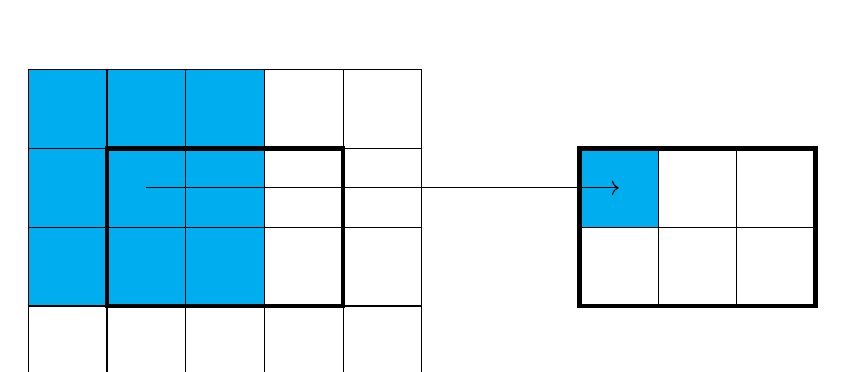
\begin{tikzpicture}
%  , fill=black!20!white
\draw [draw=black, fill=cyan] (0,1) rectangle (3,4);
\draw [draw=black, ultra thick] (1,1) rectangle (4,3);
\draw [draw=black] (0,0) grid  (5,4);

\draw [draw=black, fill=cyan] (7,2) rectangle (8,3);
\draw [draw=black, ultra thick] (7,1) rectangle (10,3);
\draw [draw=black] (7,1) grid  (10,3);

% ,very thick
\draw [->] (1.5, 2.5) -- (7.5, 2.5) ;

\end{tikzpicture}

\caption{Applying a $3 \times 3$ filter to a layer of size $4 \times 5 \times 1$. Note how the $3 \times 3$ region is reduced to a single unit and how the size of the activation map is decreased after the operation.}
\label{fig:filter}
\end{figure}


As indicated by the name, CNNs mainly consist of \textbf{convolutional layers}. Like all other layers in a CNN, a convolutional layer is three-dimensional and the depth is determined by how many filters it applies to the previous layer.  Each filter produces a two-dimensional \textbf{activation map}, as illustrated in figure \ref{fig:filter}. The values in a convolutional layer is simply the activation maps stacked on top of each other, which forms a three-dimensional structure that is passed on to the next layer.

Each scalar in the activation map comes from a weighted sum over a three-dimensional region in the previous layer over its full depth. For example a $3 \times 3$ filter applied to a layer of depth 32 has $3 \cdot 3 \cdot 32=288$ weights and one bias term.
As in MLPs, the sum is passed to a non-linear activation function such as $\tanh$.

The $3 \times 3$ regions for adjacent units are usually overlapping.
By adjusting the so called \textbf{stride} one can produce fewer output units in the activation map by ignoring some locations in between.
% It also possible to explicitly reduce or avoid such overlapping by setting a \textbf{stride} greater than one.
Thus the representational sizes of the following layers are reduced.
However, in our thesis all CNNs use the default stride, so no location is ignored.

% The activation maps for all filters are stacked together to form a three-dimensional output, which is passed to the next layer.

Because a filter uses the same weights for all sub-regions in the previous layer, the total number of parameters are dramatically reduced compared with a fully connected layer as in an MLP. Moreover, because the same filter is applied to every sub-region, the filter can detect objects regardless of their position in the image, increasing the predictive power of the network.
It also means that the same filter can be trained by images whose objects appear in different positions, which reduces the training time and makes more use of the available training data.
% Most importantly, reuse of weights increases the ability to generalize.
%it does not matter where in the input image the object is located.

\subsection{Pooling}
\begin{figure}
\centering
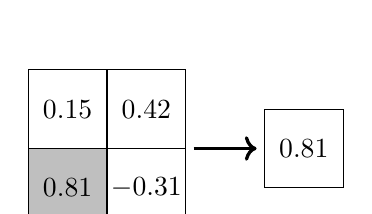
\begin{tikzpicture}

\fill[draw=black,color=lightgray] (0,0) rectangle (1,1);
\draw (0,0) rectangle (1,1) node[pos=0.5] {$0.81$};
\draw (0,1) rectangle (1,2) node[pos=0.5] {$0.15$};
\draw (1,0) rectangle (2,1) node[pos=0.5] {$-0.31$};
\draw (1,1) rectangle (2,2) node[pos=0.5] {$0.42$};

\draw (3,0.5) rectangle (4,1.5) node[pos=0.5] {$0.81$};
\draw [->,very thick] (2.1,1) -- (2.9,1) ;

\end{tikzpicture}

\caption{Example of a $2 \times 2$ max pool operation. In a $2 \times 2$ region, the largest value is chosen while the other values are ignored.}
\label{fig:maxpool}
\end{figure}


Besides filters, CNNs also use \textbf{pooling layers}, which compress the signals of the previous layer into a smaller representation without using any additional parameters.
%in order to increase the receptive field without increasing the number of parameters in the model.
% Separately for each activation map,
Pooling aggregates a two-dimensional region of units (e.g. $2 \times 2$) into a single unit, typically by taking the maximum value element-wise. A max pool operation is illustrated in figure \ref{fig:maxpool}.
The regions are non-overlapping so a $2 \times 2$ pooling layer divides the representational size by 4.
Since the representation is now smaller, the remaining computations are cheaper to perform, resulting in reduced memory usage and running time.

\subsection{Receptive field}
Since both convolutional layers and pooling layers gather information from a larger field, units in later layers in the CNN receive information from a larger \textbf{receptive field} in the input image.
% Each $2 \times 2$ pooling layer doubles the receptive field in each dimension, while every $3 \times 3$ convolutional layer increases the receptive field with 2.
Therefore, the filters in early layers typically learn to detect low-level features like edges and curves while filters in later layers can detect more complex objects like cats or faces.
By synthesizing the input image to maximize a specific filter's activation, it is possible to get an idea of what the filter has learned to recognize \cite{VisualizeCnn}.

We can calculate the size of the receptive field for each output unit by doubling the field for each $2 \times 2$ pooling layer and adding $n-1$ for each $n \times n$ convolutional layer.
If we have a network that consists of two $5 \times 5$ convolutional layers with a single $2 \times 2$ max pool layer in between, then we can compute the size $r \times r$ of the receptive field as follows:
\[
r = 4 + 2(4 + 1) = 14
\]

\subsection{Output}
At the end of the network, there are often a few fully connected layers (MLP) where the last layer represents the output of the network, for example pseudo-probabilities for different categories using softmax, as discussed previously.

\subsection{Network architecture for faster computation}

The performance of CNNs typically increases with greater width and depth, but it comes at a higher computational cost \cite{InceptionV3}. However, by choosing a good network architecture the same performance can be achieved at a substantially lower computational cost. One such guideline is to refactor large filters ($5 \times 5$, $7 \times 7$) into several small consecutive filters ($3 \times 3$). \textcite{InceptionV3} also suggest using more pooling layers early in the network as well as maintaining a balance between depth and width of the network. The representational size should also decrease slowly throughout the network without

% \textcite{InceptionV3} recommend that representational bottlenecks are avoided and that the representational size should decrease slowly after each layer.

\subsection{Zero padding}

Applying a $3 \times 3$ filter to an input image of size $10 \times 10$ will output an image of size $8 \times 8$ since there are only 8 positions in a single row where the filter can fit. For deep networks, this shrinking might cause the final representation to become too narrow.
One can pad each activation map with zeroes to instead maintain the same size, which solves the problem at little additional computional cost.

\newpage
\section{Attention models}
\label{ssec:attention}
% Since waypointing only needs high-level information in a limited domain, complete transcription is unnecessary. Instead we can use recent advances in image classification.

In contrast to CNNs, the human eye does not process the entire scene with equal precision but focuses on the most relevant parts \cite{DeepMindAttention}.
Similarly, we can let the system pay \textbf{attention} to a small part of the image at a time and successively increase the system's understanding of the image.
By choosing good locations for our attention, the important parts of the image are captured while the irrelevant parts are ignored.
This reduces the computation time for training and also increases the precision of the network.
% The process of how to select a location to focus on is called an \textbf{attention model} and is often implemented using a \textbf{recurrent neural network} (RNN).
Besides image classification, attention models have also been highly successful for image captioning \cite{AttendAndTell} and machine translation \cite{machine_translation_attention}.

% \subsection{Details}
We now describe how the attention model that was introduced by \textcite{machine_translation_attention} works in more detail.
The goal of the attention model is to produce a vector $\mathbf{z} \in \mathbb{R}^D$ that represents the entire input image by weighing different parts of the output from the encoder CNN.

The encoder output is three-dimensional but can be seen as a grid of $L$ feature vectors. Each feature vector $\mathbf{a_i} \in \mathbb{R}^D$ corresponds to a specific location in the input image. We feed each $\mathbf{a_i}$ to an MLP which produces a scalar $e_i \in \mathbb{R}$. In the paper, the decoder uses an RNN whose hidden state is also used as input to the MLP besides the feature vector $\mathbf{a_i}$.
The scalar attention weight $\alpha_i$ for each location $i$ can then be computed by taking the softmax of $e_i$ over all locations:
\[
\alpha_i = \frac{ \exp(e_i) }{ \sum_{k=1}^L \exp(e_i) }
\]

\subsection{Soft attention} \label{sssec:soft_attention}
By definition, the attention weights sum to one. A \textbf{soft attention} model computes the representative vector $\mathbf{z}$ by summing over the feature vectors $\mathbf{a_i}$, using attention as weights:
\[
\mathbf{z} = \sum_{k=1}^L \alpha_i \mathbf{a_i}
\]

\subsection{Hard attention}
A \textbf{hard attention} model instead interprets the ${\alpha_i}$ as a probability distribution over locations $i$. By sampling this distribution, $\mathbf{z}$ is chosen to be the sampled unit $\mathbf{a_i}$, ignoring the rest of the image.

\newpage
\section{CNNs in multi-digit recognition}

CNNs have not only been successful at image classification in general, but also specifically at detecting digits in images.

\subsection{Zip code detection}

Digit recognition has been studied extensively, especially for recognition of zip codes in the US postal service \cite{lecun_1989, lecun_1990}. Originally, the digits were segmented manually and linearly transformed to a fix input size of $16 \times 16$ pixels.
Each digit image was then classified using a CNN with 3 or 4 hidden layers, with $2 \times 2$ pooling between each convolutional layer.

A complete zip code recognition system locates the place of the zip code and segments the zip code into digit images \cite{zipcode_system}. The segmentation is performed by finding \textbf{connected components} (CC) in the binarized image. We discuss more about connected components and segmentation in section \ref{sec:alt_htr}.
% After binarizing the image (explained in section \ref{sssec:binarization}), a connected component.
If the CC has a high confidence in classification it is removed, otherwise it is either split or combined with adjacent CCs until a segmentation has been found where each classification has a high enough confidence. This is done by building a directed acyclic graph where each proposed segment is a node. The length of a path is defined as the product of the classification confidence for each node in the path. The best segmentation is then the path of greatest length in the graph. In order to avoid redundant computations, the segmentation can be done indirectly after the convolutional layers instead of on the input image \cite{lecun_multidigit}.

\subsection{Street view house numbers}

% TODO merge places about SVHN...

More recently, deep neural networks have achieved state-of-the-art in multi-digit recognition in street view images \cite{multidigit_streetview}. Instead of handling localization, segmentation and classification as separate tasks, they solve all of them using a single CNN with 11 layers. The output is modeled as a sequence $S$ of digits with a maximum length $N$. The sequence $S$ consists of a random variable $L=n$ for the length of the sequence and $n$ variables $S_i$, one for each digit. In order to handle images without numbers $L$ is allowed to have the value zero and in order to handle longer sequences than $N$, $L$ has a special value \textquote{greater than $N$}. For an input image $X$, the system can be trained by maximizing $\log P(S \mid X)$.
Classification is similarly done by $\argmax_S P(S \mid X)$.
% Classification is similarly done by $\text{arg\,max}_S P(S \mid X)$.
Because each variable has a very small domain, they can be implemented with independent softmax outputs.
Although this model works well for digit recognition of short sequences $N \leq 5$ as well as \textbf{optical character recognition} (OCR) in CAPTCHAs, the authors speculate that the method is not suitable for long or unbounded sequences.

Another suggested approach to digit recognition in street view is to combine CNNs with \textbf{hidden markov models} (HMMs) \cite{multidigit_streetview_CNN_HMM}. They use a sliding window to extract multiple overlapping frames on the input image, classify each frame using a CNN to either a digit or null and then feed the sequence of frame labels to an HMM.


\section{Additional topics}
Here we present some related recent progress in the field of neural networks in computer vision, although we do not directly use these results in the thesis.
Evaluation of these methods on our task is considered future work.

\subsection{Batch normalization}

An alternative to dropout was suggested by \textcite{BatchNormalization}. Besides reducing the risk for overfitting, the authors claim that it allows for a higher learning rate in deep networks and thus faster convergence.

For some network layer $\mathbf{x} = {x_1, \ldots, x_d}$, we normalize each $x_i$ to zero mean and unit variance over the current mini-batch:
\[
\hat{x_i} = \frac{x_i - E[x_i]}{ \sqrt{\text{Var} [x_i]} }
\]

We then use two learned parameters $\gamma$ and $\beta$ to instead output $z_i$:
\[
z_i = f_{BN}(x_i; \gamma, \beta) = \gamma \hat{x_i} + \beta
\]

The batch normalization can either be applied before or after the activation function. The authors suggest that the best result is achieved by applying the batch normalization before the non-linear activation $g$ but after the weights $w_{ij}$ and bias $b_i$:
\[
v_i = g\left( f_{BN}\left( b_i + \sum_j w_{ij} u_j; \gamma, \beta \right) \right)
\]

\subsection{Visual-semantic alignment}

% Another way to model regions in the input is by using a R-CNN which have also been very successful at image captioning

Although \textcite{AttendAndTell} successfully used attention models for image captioning,
an alternative successful method instead uses a \textbf{region convolutional neural network} (R-CNN) as encoder \cite{VisualSemanticAlignment}.
The original R-CNN method works by proposing 2000 regions in the image that are the most likely to contain an object \cite{RCNN}. Each region is then fed to a regular CNN for encoding before classification.

Since many regions overlap, it is unnecessary to compute the convolutions for them independently \cite{FastRCNN}. Instead the entire input image is processed through the CNN once and the feature vector of each region is extracted from the resulting activation map. After this improvement, the bottleneck is selecting the regions \cite{FasterRCNN}. By making a neural network to select regions from the activation map instead of from the image, the computation speed can be significantly reduced. However, this requires the training data to contain bounding boxes for the objects to detect.

For the case of image captioning, the correspondences between words and regions in the image is unknown so this relationship is modeled by latent variables \cite{VisualSemanticAlignment}. Because the true association between labels and regions is unknown we say that these labels are weak.

\subsection{Spatial transformer networks}

Another exciting innovation for CNNs is \textbf{spatial transformer modules} \cite{SpatialTransformerNetworks}. Each spatial transformer module dynamically finds an interesting part of the input image and transforms it by spatial operations such as scaling, cropping and rotation. For example in handwriting transcription, such a module could in theory locate and normalize words in the input image. Spatial transformer networks has been proven to work well for both digit recognition and image classification.

\subsection{Spatial pyramid pooling}

Convolutional layers and pooling layers can handle input images of changing sizes since the filters just slide over the entire image, so the size of the output matches the input.
However, because the last network layers are fully connected, they can only handle input of a fixed size. A common solution to this is to rescale or crop the input \cite{FornesCnnCategorization}. If the input consists of segmented images of handwritten words, then cropping will cut away critical information, while rescaling would risk distorting the handwriting beyond recognition. A proposed solution to this is using a layer of \textbf{spatial pyramid pooling} (SPP) \cite{FornesCnnCategorization}.

% \subsection{Residual networks}

% cite Microsoft ResNet for architecture of Residual modules. There are also residual networks of residual networks.

% TODO check page here!



\section{Method}

\subsection{Network architecture}


\begin{figure}
\centering

% TODO should mention sizes! Maybe represent decoder output differently.

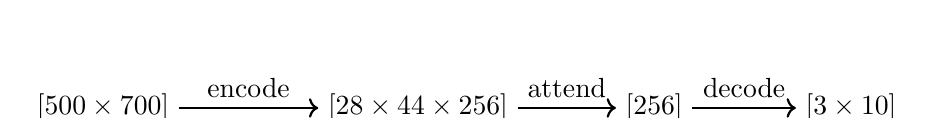
\begin{tikzpicture}
% 900, 1500, 1
% 28, 44, 256
% 1, 1, 256
% 3, 10

    \node (input) at (0,0) {$[500 \times 700]$};
    \node (encoded) at (4, 0) {$[28 \times 44 \times 256]$};
    \node (attended) at (7, 0) {$[256]$};
    \node (decoded) at (9.5, 0) {$[3 \times 10]$};

%   \pic [fill=cyan, draw=blue] at (-1,0) {annotated cuboid={width=1, height=900, depth=1500}};
%   \pic [fill=cyan, draw=blue] at (4,-0.5) {annotated cuboid={width=256, height=28, depth=44}};
%   \pic [fill=cyan, draw=blue] at (7,-0.5) {annotated cuboid={width=256, height=1, depth=1}};
%   \pic [fill=cyan, draw=blue] at (9,1.5) {annotated cuboid={width=1, height=10, depth=3}};

  \draw [->,thick] (input) -- node [above] {encode} (encoded);
  \draw [->,thick] (encoded) -- node [above] {attend} (attended);
  \draw [->,thick] (attended) -- node [above] {decode} (decoded);

\end{tikzpicture}

\caption{Overview of how the data flows in the proposed network. First the encoder produces a matrix of feature vectors, each corresponding to a different but overlapping location in the input image. Secondly, the attention aggregates the feature vectors into a single feature vector. Lastly, the decoder produces three softmax outputs, one for each digit.}
\label{fig:sys_overview}
\end{figure}


We now describe the different parts of the proposed network. See figure \ref{fig:sys_overview} for an overview of how the different parts of the network interact.

\subsubsection{Experiments}
% TODO: write here or somewhere completely different?

\subsubsection{Encoder}

\begin{figure}
\centering

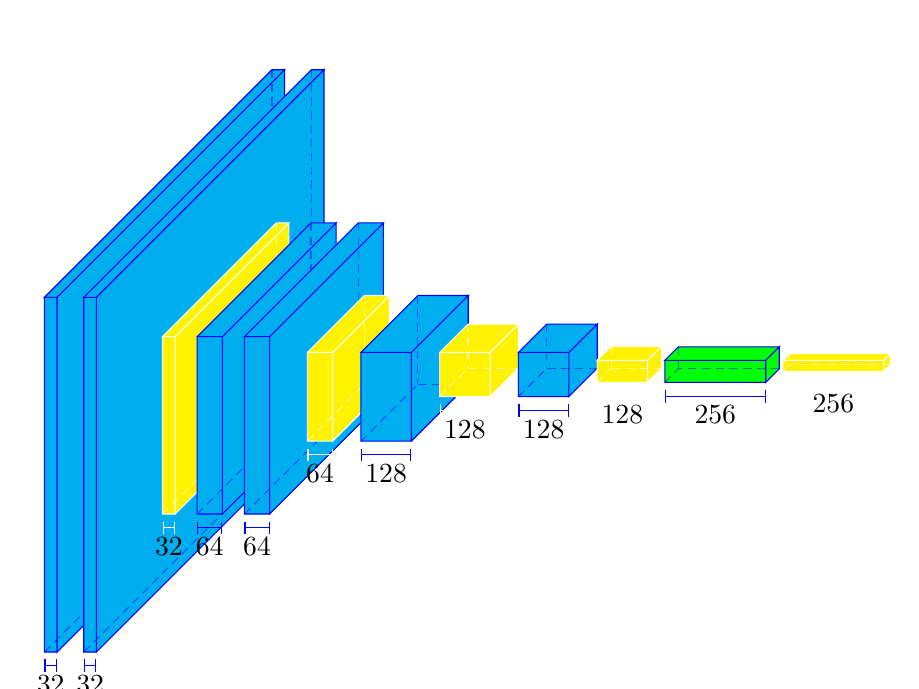
\begin{tikzpicture}
% (1, 900, 1500, 1)
% (1, 450, 750, 4)
% (1, 225, 375, 16)
% (1, 225, 375, 32)
% (1, 112, 187, 32)
% (1, 112, 187, 128)
% (1, 56, 93, 128)
% (1, 56, 89, 256)
% (1, 28, 44, 256)

%   \pic {annotated cuboid};
  \pic [fill=cyan, draw=blue] at (0,0) {annotated cuboid={width=32, height=900, depth=1500}};
  \pic [fill=cyan, draw=blue] at (0.5,0) {annotated cuboid={width=32, height=900, depth=1500}};

  \pic [fill=yellow, draw=white] at (1.5,-0.5) {annotated cuboid={width=32, height=450, depth=750}};
  \pic [fill=cyan, draw=blue] at (2.1,-0.5) {annotated cuboid={width=64, height=450, depth=750}};
  \pic [fill=cyan, draw=blue] at (2.7,-0.5) {annotated cuboid={width=64, height=450, depth=750}};

  \pic [fill=yellow, draw=white] at (3.5,-0.7) {annotated cuboid={width=64, height=225, depth=375}};
  \pic [fill=cyan, draw=blue] at (4.5,-0.7) {annotated cuboid={width=128, height=225, depth=375}};

  \pic [fill=yellow, draw=white] at (5.5,-0.7) {annotated cuboid={width=128, height=112, depth=187}};
  \pic [fill=cyan, draw=blue] at (6.5,-0.7) {annotated cuboid={width=128, height=112, depth=187}};

  \pic [fill=yellow, draw=white] at (7.5,-0.8) {annotated cuboid={width=128, height=56, depth=93}};
  \pic [fill=green, draw=blue] at (9,-0.8) {annotated cuboid={width=256, height=56, depth=89}};

  \pic [fill=yellow, draw=white] at (10.5,-0.8) {annotated cuboid={width=256, height=28, depth=44}};

%   \pic [fill=magenta, text=blue, draw=blue] at (5,0) {annotated cuboid={width=2, height=50, depth=30}};
%   \pic [fill=green, text=green!50!black, draw=green!25!black] at (5,-2) {annotated cuboid={width=6, height=20, depth=15, units=mm}};
%   \pic at (1,-3) {annotated cuboid={width=150, height=200, depth=250, scale=.01, units=m}};
%   \pic [fill=cyan, text=blue!75!cyan, draw=blue!75!cyan] at (-3,-2) {annotated cuboid={width=15, height=18, depth=13.5, units=}};
\end{tikzpicture}

\caption{Proposed architecture for the encoder. Convolutional layers are blue (3x3) and green (1x5) while max pool layers are yellow (2x2).
The number below each layer indicate the depth of the layer.}
\label{fig:encoder}
\end{figure}


For encoder, we use a CNN with 7 convolutional layers with additional pooling layers, see figure \ref{fig:encoder}.
% We experimented with several different variations in number of convolution layers, pooling layers and layer depths before choosing this model.
Two consecutive 3x3 convolutional layers is a refactoring of a single 5x5 layer as suggested by \cite{InceptionV3}. Thus, the first four convolutional layers correspond to two 5x5 convolutional layers with pooling, similar to the original single digit CNN classifier \cite{lecun_1989} but with greater depth.

The number of pooling layers, number of convolutional layers and depth per layer were determined experimentally. The final encoder design, as in figure \ref{fig:encoder}, is somewhat similar to the encoder used in \cite{FornesCnnCategorization} except that we use more aggressive pooling. This is necessary because in our work, we input images of entire pages while \cite{FornesCnnCategorization} classify word images which presumably are much smaller.

%The first four layers correspond closely to the original single digit classifier CNN \cite{lecun_1989} with the exception

% The number of layers and their depth was determined experimentally on the synthesized dataset using previous work as starting point \cite{FornesCnnCategorization}.

% TODO describe experiments.



\subsubsection{Attention model}

Another major difference between our work and \cite{FornesCnnCategorization} is that although we both use variable input size, they use \textbf{Spatial pyramid pooling} while we apply a soft attention model as presented in \cite{AttendAndTell}. Like we discussed previously in \ref{ssec:attention}, the encoder output can be seen as a list of feature vectors $\mathbf{a_i} \in \mathbb{R}^D$ which correspond to different but overlapping locations. The number of produced feature vectors depends on the size of the input image. We will see that this attention model aggregates all feature vectors $\mathbf{a_i}$ into a single fixed size vector $\mathbf{z} \in \mathbb{R}^D$.

The attention model consists of a multilayer perceptron which for each feature vector $\mathbf{a_i}$ computes a salience score $e_i$:

\[
e_i = f_\text{MLP}(\mathbf{a_i})
\]

Note that this MLP does not have access to any information about the corresponding location of $\mathbf{a_i}$, thus the network must learn to recognize important parts by looking at the encoded features alone instead of learning to always look at a certain position in the input image. This is especially important for population records where the relevant information can be in different locations depending on scribe and time period.

As discussed, we normalize the $e_i$ into $\alpha_i$ by computing the softmax. Then we use the attentions $\{\alpha_i\}$ as weights over the feature vectors:

\[
\mathbf{z} = \sum_{k=1}^L \alpha_i \mathbf{a_i}
\]

Note that the spatial information about where in the image $\mathbf{z}$ comes from is lost in this sum. So just like the attention MLP, the decoder also becomes invariant to the object's position in the input image.

\subsubsection{Decoder}

The decoder employs an MLP for classifying the aggregated feature vector $\mathbf{z}$ from the attention model.
If $\mathbf{z}$ had a variable length, then we would need a different number of weights in the MLP for each different input size. Since the attention model produces a fixed size output independent of input size we avoid the problem of variable number of parameters.

The proposed MLP consist of one fully connected layer of $1024$ neurons with dropout as well as three parallel readout layers, each with a size of $10$ neurons. The three separate outputs correspond to one digit each.

To compute the probability for a 3-digit sequence we take the cartesian product of the three readouts: (0,0,0) -- (9,9,9) and remap them to 000 -- 999, or in the case of years, to 1000--1999.

\subsection{Pre-training}
\subsection{Labeling}
\subsection{Training}
\subsection{Evaluation}


% TODO should technologies/implementation be described in a different section?
% Is it at all relevant to discuss about Tensorflow?
\subsection{Tensorflow}
% TODO Mention GPU acceleration here or in section about neural networks?

\subsection{Hardware}
% TODO Mention hardware and training time .

\chapter{Results and discussion}

\textit{
In the previous chapter we described our main model and training procedure as well as some alternatives.
In this chapter we describe the numerical results of our implementation of the main model on two datasets, one synthetic dataset created from MNIST and the much more difficult Swedish population records. We also perform several experiments where we change the model configuration or training procedure and observe the effect on either or both datasets.
Hopefully, our observations can be instrumental in
% TODO: instrumental? Rephrase?
designing future encoder-decoder networks.
}

\section{Simulations on synthetic data} \label{sec:simulations}

Since the images of the Swedish records are so large, we decided to create a simpler dataset, which would be faster to train on, so we could quickly iterate on the network architecture. Here we describe the synthetic dataset we created as well as some observations from altering the network configuration.

\subsection{Four-digit MNIST}


\begin{figure}
    \centering
    \begin{subfigure}[b]{0.45\textwidth}
        \centering
        
\includegraphics[scale=2.0]{resources/mnist4.jpg}
        \caption{Four digits without noise.
        %, size $112 \times 28$.
        }
        \label{fig:mnist4}
    \end{subfigure}%
    \begin{subfigure}[b]{0.45\textwidth}
        \centering
        
\includegraphics[scale=2.0]{resources/random_pad.jpg}
        \caption{Random position and dot noise.
        %Four digits with noise.
        %at a random position inside a box of $168 \times 56$ with dot noise.
        }
        \label{fig:mnist_random_pad}
    \end{subfigure}
    \caption{Two examples of generated synthetic data from MNIST.}
\end{figure}

For our early experiments we created a synthetic dataset with small images of four-digit sequences.
Each image was a concatenation of four independently randomly selected digit images from MNIST \cite{MNIST_orig}, where the first digit was always a one. See figure \ref{fig:mnist4} for an example. The resulting image was then a fixed size of $28 \times 112$ pixels.
%, compared to $900 \times 1500$ or more for the downsampled Swedish records.
% which is very much smaller than the images of the Swedish records.
Because the images were so small, it took a much shorter time to train and evaluate different models on the synthetic dataset than on the Swedish population records, whose images were very large.

Several models performed very well on this task, one of them achieving $94\%$ accuracy after 10,500 CPU seconds of training. These models are discussed further in section \ref{sssec:exp_encoder}.

\subsection{Noisy MNIST}

In order to make the synthetic data a little bit more difficult to classify and more similar to the Swedish dataset, each four-digit image was placed at a random position in a larger image whose pixel values were zero, that is no ink.

When putting the four-digit image at a fixed position instead of a random position, one model learned to encode the distance from the left side of the image, which is quite interesting considering that neither the attention model nor the decoder had any explicit access to spatial information.
When adding $100$ additional zero-pixels to the right of the image, the accuracy dropped from $85\%$ to $80\%$. However, when adding $4$ zero-pixels to the left, the accuracy dropped to only $1\%$. We attribute this sudden accuracy loss to the difficulty of identifying which digit to keep and which to ignore. Since we are training on four-digit images but only expect the last three, the model must learn to find but ignore the first digit.
Since the year can appear at any position in the Swedish data, the simulations should also vary the position of the digits. Therefore, we must use random positions instead of fixed positions for the synthetic data.

Finally, we applied dot-noise to the image by:
(1) inverting the image so that the background is represented by one instead of zero,
(2) multiplying each pixel value with a random number drawn independently uniformly from $[0.6, 1.0]$ and
(3) inverting the image back again.
This corresponds to adding a random but small amount of ink to each pixel in the image.

An example image with dot noise and random position can be seen in figure \ref{fig:mnist_random_pad}. The models were evaluated on the image size $56 \times 168$ pixels, like in the figure.


\subsection{Network depth and width} \label{sssec:exp_encoder}

By running a time trace on the training operation, we saw that the majority of the training time was spent on applying and updating the encoder network. In order to reduce training time we performed the following experiments to design a more efficient encoder network while maintaining a good accuracy on the simulation tasks.
% TODO: insert graph?

% By counting the number of trainable parameters in the model we observed that the majority of parameters are contained by the MLPs in the attention and decoder model.

\subsubsection{Simulations on noise-free data}

Earlier in section \ref{sec:method_architecture} we presented a model architecture that we now refer to as DEP. We will come back to this model soon. In our initial experiments however we used another model for baseline, which we call DE. The DE encoder consisted of four blocks where the first three blocks contained two $3 \times 3$ convolutional layers and one $2 \times 2$ pooling layer. The last block contained a single $1 \times 5$ convolutional layer and one $1 \times 2$ pooling layer.
The main difference between DE and DEP is that DEP used one additional pooling layer between the two consecutive convolutional layers in the third block.
% The only difference between DEP and DE is that DEP had one additional pooling layer between two convolutional layers near the end of the encoder.
We will see that this small difference had a great impact on accuracy and running time.


\begin{figure}
    \centering
    \begin{subfigure}[c]{1.0\textwidth}
        \centering    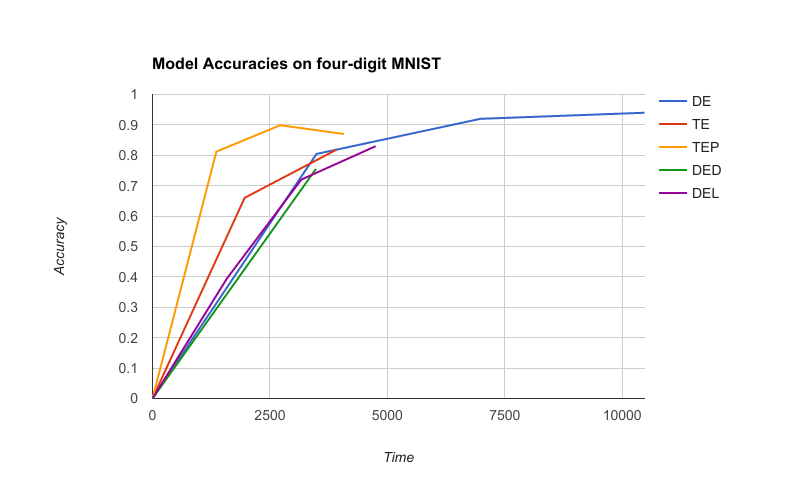
\includegraphics[scale=0.5]{resources/mnist_4_graph.png}
        \caption{Four-digit MNIST without noise.}
        \label{fig:mnist_early_models}
    \end{subfigure}
    \begin{subfigure}[c]{1.0\textwidth}
        \centering
        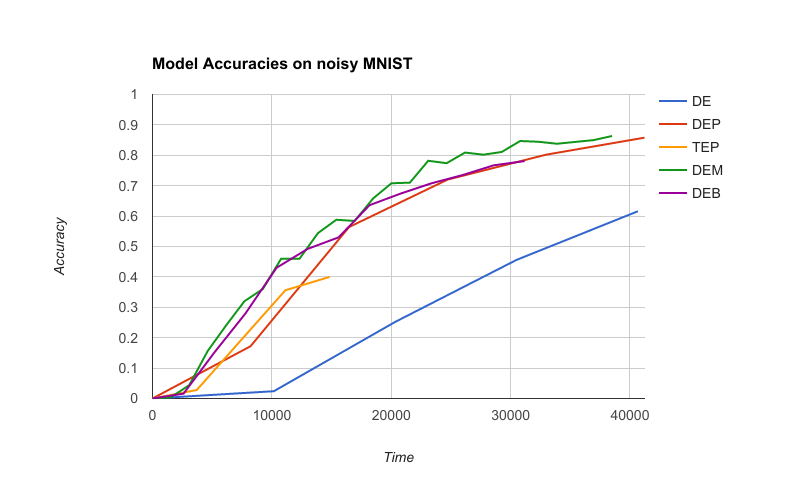
\includegraphics[scale=0.5]{resources/model_experiments.png}
        \caption{Noisy MNIST.}
        \label{fig:mnist_models}
    \end{subfigure}
    \caption{Plot of accuracy vs training time measured in CPU seconds for several models. Each data point comes after one epoch of training.}
\end{figure}


In figure \ref{fig:mnist_early_models} we can see the resulting accuracy over training time of the different variations of the DE model.
All configurations used cartesian loss (defined in section \ref{sssec:cartesian}) and soft attention (defined in section \ref{sssec:soft_attention}).

% For baseline we use a model called DE, which is rather similar to the model presented earlier in section

% The DE model was used as baseline with an encoder that had 7 layers and an output depth of 256. It is very similar to the DEP encoder illustrated in figure \ref{fig:encoder} except that it used one less pooling layer.

The model called DED was the same DE except that the decoder depth was halved from 1024 to 512. In figure \ref{fig:mnist_early_models} we can see that doing so had little impact on the accuracy and training time.

In another experiment, which we refer to as DEL, we halved the depth of every encoder layer. Halving the depth of every encoder layer halves the representational size in the encoder and consequently halves the training time. However, simplifying the encoder like this also seems to have limited its learning capability. In fact, it had about the same accuracy per training time as the DE model.

% When halving the depth of the DE decoder from 1024 to 512, (DED) had little impact on this task.
% Halving the number of filters in every layer (DEL) halved the training time per epoch but also halved the learning rate, so in the end its performance was about the same.

% The TE model was identical to DE except that it used fewer convolutional layers. More precisely, the DE encoder started with $\langle C,C,P,C,C,P \rangle$ while TE started with $\langle C, P, C, P \rangle$, where $C$ stands for $3 \times 3$ convolution and $P$ stands for $2 \times 2$ max pooling.

% In both the DE model and the DEP model, the encoder had two consecutive convolutional layers at two places in the beginning of the encoder. These double layers in the DEP model can be seen in figure \ref{fig:encoder}.
In order to reduce the training time, we experimented with
simplifying the DE encoder by removing the second convolutional layer in each of the first two blocks. We call this thinner model TE.
% removing two convolutional layers so that there would be no consecutive convolutional layers. So in the model we call TE, every second layer in the encoder was a max pool layer.
Similarly to the model DEL described above, where we simplified the encoder by halving the depth of each layer, both training time and accuracy was reduced. When plotting accuracy against training time in figure \ref{fig:mnist_early_models}, we see that just like DEL, the TE model was comparable to DE.

We also tested a variant to TE where an additional pooling layer was added between the two convolutional layers in the third block. So in this new model, which we call TEP, every second layer is a pooling layer.
Compared to TE, the TEP model learned much quicker. However, TEP started to overfit after hitting $90\%$ accuracy while the baseline model DE continued to improve until $94\%$.

% When adding an additional pooling layer (TEP) to the thinner model (TE), learning increased very rapidly for the first two epochs. However, it started to overfit after hitting $90\%$ accuracy, while the accuracy of the baseline model (DE) continued to rise to $94\%$.

In summary we can see that models with smaller representational size achieves about the same accuracy given the same amount of training time, although the heavier models seem to have higher potential in the long run. Another observation is that additional pooling can greatly increase the learning rate in the beginning of training.

% The learning rate on the simpler four-digit MNIST dataset for different some possible configurations of the encoder.

% By training on the simpler four-digit MNIST dataset without noise,
%we made several observations.
% We experimented on various configurations of encoder and decoder depth and width.
% we found that increasing the width of the decoder's hidden layer from 512 to 1024 had a very small impact on the training time while increasing accuracy. Decreasing the number of layers in the encoder from 7 to 5 decreased the accuracy somewhat but increased training time considerably. Halving the encoder width halved the training time but also decreased accuracy. Adding a pooling layer at the end of the encoder resulted in a higher accuracy after the first epoch and reduced training time. The effect of an extra pooling layer can be seen by comparing the models TE and TEP in figure \ref{fig:mnist_early_models}.

\subsubsection{Simulations on noisy data}

The best configurations so far were evaluated on the more difficult synthetic dataset with random positions and noise. Figure \ref{fig:mnist_models} contains a comparison between some variations of encoder configurations on the noisy MNIST dataset.
By comparing this graph to figure \ref{fig:mnist_early_models}, we can see that using larger input images, placing the digits at a random position and adding noise makes the problem much more difficult. Training a single epoch takes almost three times as long and the increase in accuracy per epoch is reduced considerably.
%Note that for the same model, we needed to train more than 4 times longer to get the same accuracy as on the simpler synthetic dataset.

The three best configurations (DEP, DEB, DEM) achieved very similar results considering the test accuracy vs training time. These three configurations had the same number of encoder layers but different depth of each layer.

The heaviest encoder DEP is illustrated in figure \ref{fig:encoder}.
Because it had the most number of filters, the training time for each epoch was much longer than for the other two alternatives.
% For this encoder the representational size of the input decreases exponentially for each pooling layer: 32, 16, 8, 4, 2.
Since each pooling layer divides the representational size by four and the number of filters in this model doubles after almost every pooling layer, the representational size decreases is halved after most pooling layers.

While the representational size decreases for DEP, as recommended by \textcite{InceptionV3}, the DEM encoder was designed to keep the representational size as constant as possible from the start.
This was done by reducing the layer depth to a minimal amount, with only 4 filters at the input layer instead of 32.
As we can see in figure \ref{fig:mnist_models}, the training time for each epoch was much faster although the actual learning over time was almost the same as for the DEP model.

The third competing encoder DEB was a middle ground between DEP and DEM, designed to have a very slowly decreasing representational size.

\subsubsection{Wider encoders are more robust to varying input size}


\begin{figure}
    \centering
    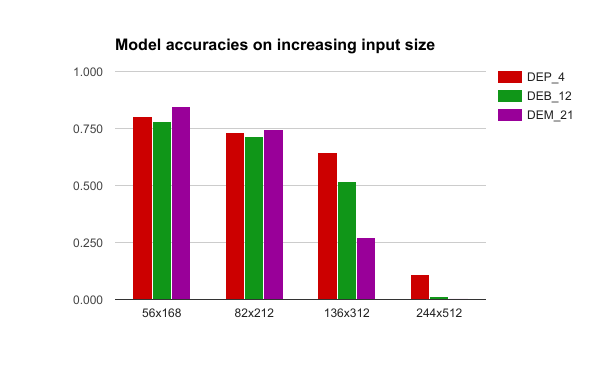
\includegraphics[scale=0.5]{resources/mnist_resilience.png}
    \caption{Noise resilience... TODO}
    \label{fig:mnist_resilience}
\end{figure}

When increasing the size of the generated synthetic images without retraining the models, the accuracy of the DEP model was relatively stable even for the double width and height but dropped for larger input. The two lighter models, DEB and DEM, were less robust to this change in input; see figure \ref{fig:mnist_resilience}.

The attention model is responsible for choosing the correct location in the input image. The receptive field of output units in the three configurations were the same and the architecture of the attention model was identical. The background noise was also identical. So although the attention model worked well for a smaller image, it is not sure it may work as well for a larger image where the background is the same.
% One possible reason for this is that the soft attention for all locations must sum to one. Since there are more locations to choose from, the weight on the correct location decreases.
Remember that the attention model does not know how many locations there are but outputs a salience score for each location independently. Since we use the softmax of these salience scores, the resulting attention weights must sum to one. So the more locations there are, the more the attention risk to spread out over noisy locations. To counter this, the attention model would have to be even more aggressive to separate background noise from useful signals. For hard attention however, only the most promising location is kept and the rest are ignored. So a model trained with hard attention should be more resilient to increased image size. We discuss more about attention later in section \ref{sssec:result_attention}.

We see that the more filters a model has, the more stable it is to change. Hence we believe that although on a single task the three configurations performed comparatively, the heavier model generalizes better in the long run.

% We attribute this resilience to noise to detecting more features in the input, some of which are better preserved after adding the noise.


% We argue that the heavier model, DEP, with its additional filters can detect more features in the input

% The lightest encoder (DEM) was designed to have the same representational size as DEP at the end of the encoder but decreasing the number of filters in the beginning in order
% keeping the representational size as constant as possible from the start by using fewer filters, in contrast to the advice from \textcite{InceptionV3}.


\section{Experiments on Swedish population records} \label{sec:experiments}

In this section we present and discuss our model with variations on the Swedish population records.
% metrics of different models and training
% comparisons we made between different models on the Swedish population records.

\subsection{Setup}
 Here we describe the platform on which we evaluated the models.

\subsubsection{Downsampling}
The images of the Swedish population records had a high resolution so they were downsampled with a ratio of 8. For example instead of having a size of $4688 \times 6360$ an image would have the size to $586 \times 795$. Because the images have different sizes, in each batch the images were padded with zeroes to get the same size as the largest image in the batch.

\subsubsection{Implementation}
The models were implemented in Tensorflow \cite{Tensorflow}, which is a popular open-sourced machine learning framework. The implementation\footnote{\url{https://github.com/HalfLeif/CNN_doc_extraction}} is freely available on Github.

\subsubsection{Hardware}
We trained the models on 3 threads on a single Intel(R) Core(TM) i7-4770K @ 3.50GHz. Training a single epoch of Swedish population records took about 28 hours. It would be faster to train using more threads or GPU acceleration but we were constrained by limited access to hardware.


\subsubsection{Pre-training}

All experiments in this section start with a pre-trained model already. Most of them use a model we refer to as the \textbf{Base model}. The Base model used the DEP encoder and was trained using soft attention and cartesian loss for 5 epochs on the noisy MNIST and then for 16 epochs on the Swedish population data. Thus it had an accumulated training time of more than 4,200,000 cpu-seconds or more than 2 weeks on our hardware.
% noisy MNIST DEP-5: 41,217 cpusec ?
% 16 epochs of SweDEP: 264775*16 cpusec = 4,236,400
% SUM:
The Base model had an accuracy of $8.39\%$ on the main test set and an accuracy of $2.11\%$ on the second test set.

Optimally, the model variations should be retrained from scratch but doing so would simply take too long time.
Instead, we present the observed accuracies as an indication of whether the variation was helpful or not.
% Since the models were heavily pre-trained with a different configuration, we present our observations as a lower bound to the potential accuracy of each variation.

% that pre-trained on the noisy MNIST for 5 epochs which was then trained on the Swedish population data

% The experiments in this section were performed after training the model for many epochs on the Swedish data already. Optimally we would want to retrain the model from scratch for each alteration but doing so would take too much time. Thus we can only provide a lower bound for the accuracy of the altered models.


\subsection{Independent digits vs cartesian loss} \label{sssec:ind_digits}

We now compare using the independent digit loss presented in section \ref{ssec:method_loss} against the cartesian loss introduced in section \ref{sssec:cartesian}.
% TODO: check in notes for results on MNIST data.
Training the DEP configuration from scratch on the noisy MNIST data using either loss function gave very similar results although the training time was slightly longer for cartesian loss.

For the Swedish population records, the Base model used cartesian loss already. When training one additional epoch using the independent digit loss, the test accuracy dropped from $8.39\%$ to $7.2\%$. However, when training the model for another six epochs we reached the test accuracy of $8.98\%$. This model we refer to as  Base2 because some of the following models were trained from this model.

\subsection{Multi-year vs single-year loss} \label{ssec:result_multiyear}

Both the cartesian loss and independent digit loss discussed above only used a single year from the label. We suggested another loss function in section \ref{sssec:alt_multiyear} that takes into account the full year interval in the label by averaging the loss function over all years in the label interval. Now we compare using the multi-year vs the single-year version of independent digit loss.

As mentioned above, when changing the loss function for the Base model to single-year independent digit loss for one epoch, the accuracy dropped from $8.39\%$ to $7.2\%$. However, when instead changing it to the multi-year version, the accuracy dropped even further to $7.07\%$. When training with multi-year loss from  Base2 for four epochs, the test accuracy dropped from $8.98\%$ to $7.58\%$

Although the test accuracy for the multi-year model decreased, the accuracy on the second test set increased from $2.35\%$ to $2.75\%$. This is the best result we have achieved on the second test set, which tests the model on completely new books from other regions.

In conclusion, the multi-year loss decreased the accuracy on the main test set but improved the model's ability to generalize to new collections.
One possible cause for this may be that multi-year loss makes the network focus more on the handwritten digits instead of the handwriting. However, when comparing the attention for the two models on the same images they look quite similar.


\subsection{Simplifying the training data}

When a page contains multiple valid years, our single-year loss function only rewards finding the highest year and penalizes all other years, including valid ones.
In our previous experiment, we attacked this problem of miss labeling in our training data by making a loss function that takes into account all the years in the label. In this experiment, we instead try to estimate the impact of miss labeling by only training on images that have a single year in it. Here we again the use single-year independent digit loss function.

After training for one additional epoch beyond the  Base2 model, the test accuracy dropped from $8.98\%$ to $8.83\%$.
After another five epochs, we reached the highest seen test accuracy of $9.54\%$. On the other hand, the accuracy on the second test set was an all-time low at $1.42\%$.

\subsection{Soft vs hard attention} \label{sssec:result_attention}

So far, all reported models have used soft attention. Hard attention uses the same network, the only difference is that instead of doing a weighted sum over the encoded locations, we choose one of them. In previous work, the hard attention has seen the attention weights as a distribution over the location and samples that distribution. In our work however, we simply choose the location with highest attention weight.


\begin{figure}
    \centering
    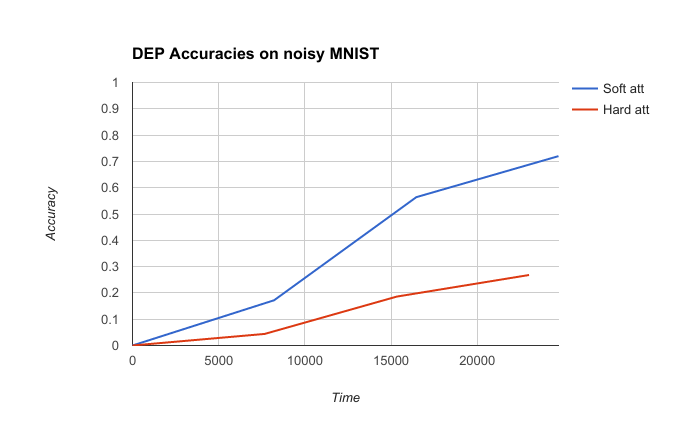
\includegraphics[scale=0.6]{resources/soft_vs_hard.png}
    \caption{The DEP model learns much faster with soft attention on the noisy MNIST dataset. Plot of accuracy vs training time measured in CPU seconds.}
    \label{fig:attention_mnist_graph}
\end{figure}


When training the DEP model with hard attention from scratch on the noisy MNIST data for one epoch, we only got a test accuracy of $4.4\%$ instead of $17.2\%$.
In figure \ref{fig:attention_mnist_graph} we can see how much quicker the DEP model learns to recognize digit sequences using soft attention.


\begin{figure}
    \centering
    \begin{subfigure}[c]{0.45\textwidth}
        \centering    
\includegraphics[scale=2.0]{resources/MNIST_soft_att/1177_att.jpg}
        \caption{Soft attention in white on the image to the right. It correctly focused more to the bottom and left.}
        % \label{fig:mnist_early_models}
    \end{subfigure} \quad %
    \begin{subfigure}[c]{0.45\textwidth}
        \centering
        
\includegraphics[scale=2.0]{resources/MNIST_soft_att/1177_correct.jpg}
        \caption{The image was correctly classified as 1177.}
        % \label{fig:mnist_models}
    \end{subfigure}
    
    \vspace{1em}
    
    \begin{subfigure}[c]{0.45\textwidth}
        \centering    
\includegraphics[scale=2.0]{resources/MNIST_hard_att/1281_att.jpg}
        \caption{Hard attention in white of the image to the right. The attention only captured part of the number.}
        % \label{fig:mnist_early_models}
    \end{subfigure} \quad %
    \begin{subfigure}[c]{0.45\textwidth}
        \centering
        
\includegraphics[scale=2.0]{resources/MNIST_hard_att/1281_fail_1031.jpg}
        \caption{Input image with label 1281, it was incorrectly classified as 1031.}
        % \label{fig:mnist_models}
    \end{subfigure}
    \caption{Examples of soft and hard attention applied to noisy MNIST images with sizes $312 \times 136$.}
    \label{fig:attention_mnist}
\end{figure}


In figure \ref{fig:attention_mnist} we can see how the soft attention successfully captured the year by putting together information from several locations. In the same figure, the hard attention fails because it can only see some of the digits.


\begin{figure}
    \centering
    \begin{subfigure}[c]{1.0\textwidth}
        \centering    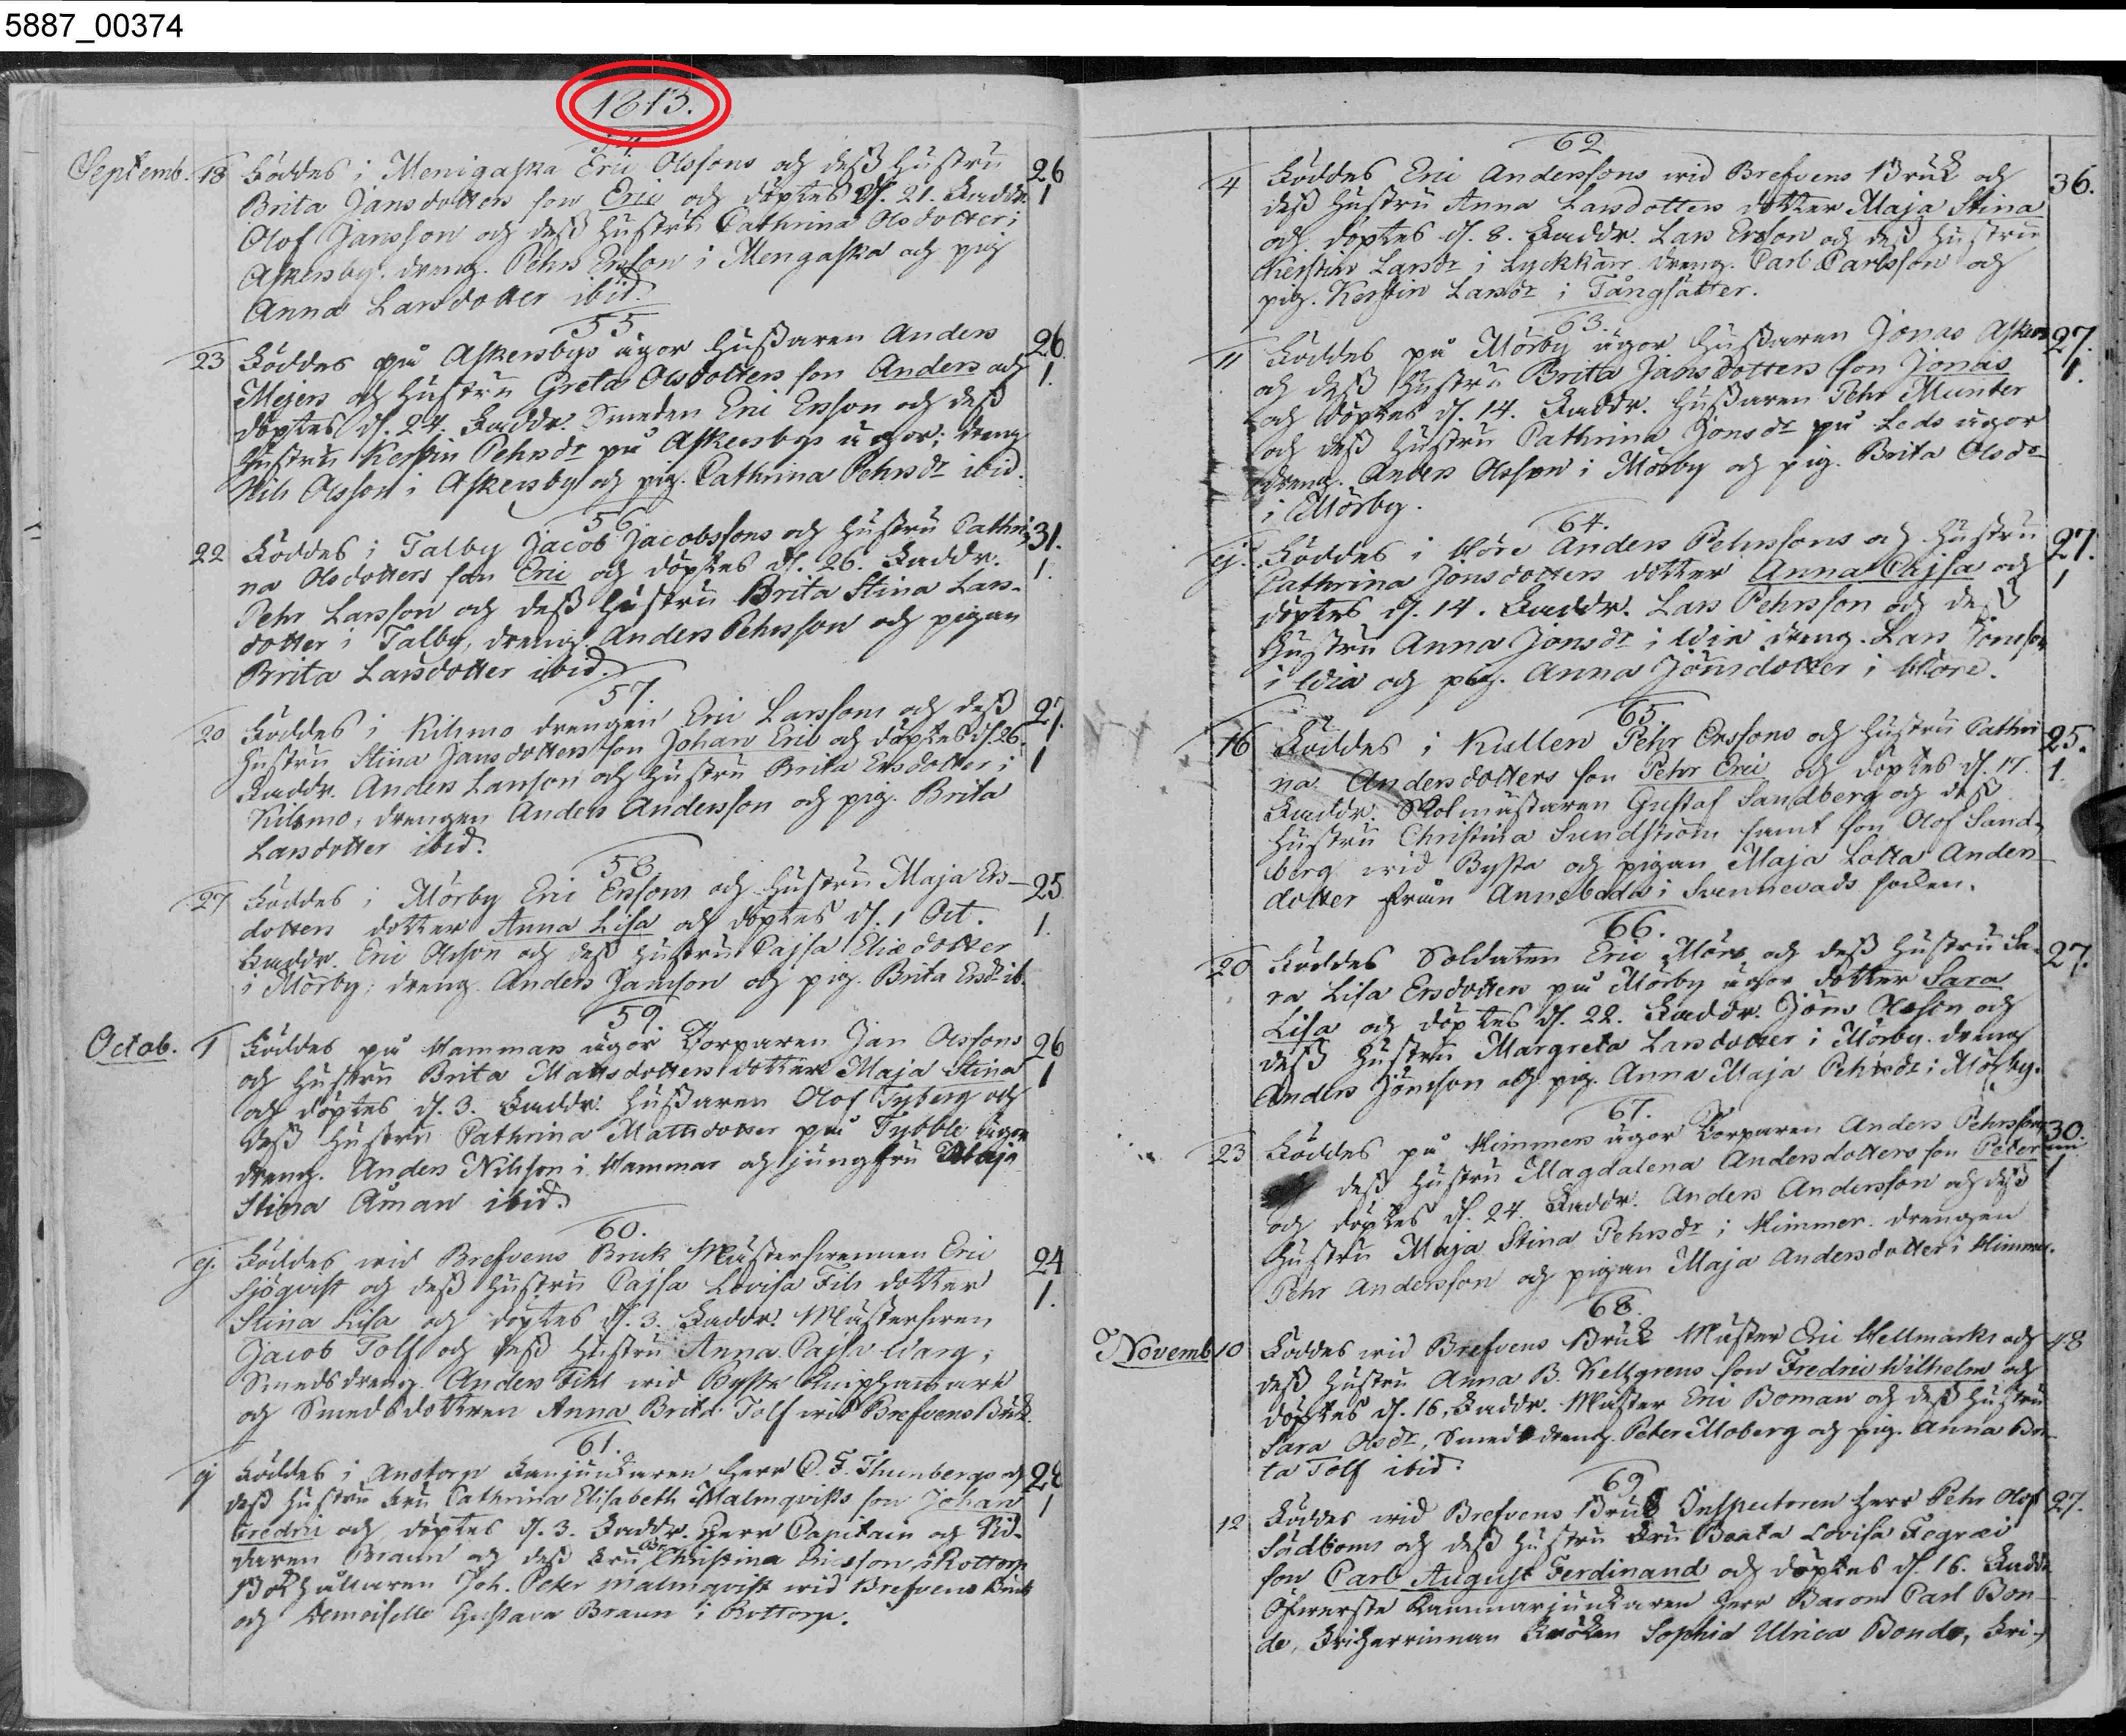
\includegraphics[scale=0.56]{resources/SWE_attention/S3HT-64P3-T61.jpg}
        \caption{The correct year is 1813; it is emphasized in the picture with ellipses.}
    \end{subfigure}
    
    \vspace{1em}
    
    \begin{subfigure}[t]{0.45\textwidth}
        \centering
        
\includegraphics[scale=1.0]{resources/SWE_attention/SoftAtt/att_S3HT-64P3-T61.jpg}
        \caption{The base model correctly classifies the image as 1813. The attention correctly focuses on the year as well as on some handwriting.}
    \end{subfigure} \quad %
    \begin{subfigure}[t]{0.45\textwidth}
        \centering    
\includegraphics[scale=1.0]{resources/SWE_attention/HardAtt/att_S3HT-64P3-T61.jpg}
        \caption{The hard attention model predicts the page as 1899 because it is looking at the wrong location.}
    \end{subfigure}
    
    \caption{An image from the main test collection. The page comes from the book Asker C:4 in the Örebro collection.}
    \label{fig:attention_dep_T61}
\end{figure}


\begin{figure}
    \centering
    \begin{subfigure}[c]{1.0\textwidth}
        \centering    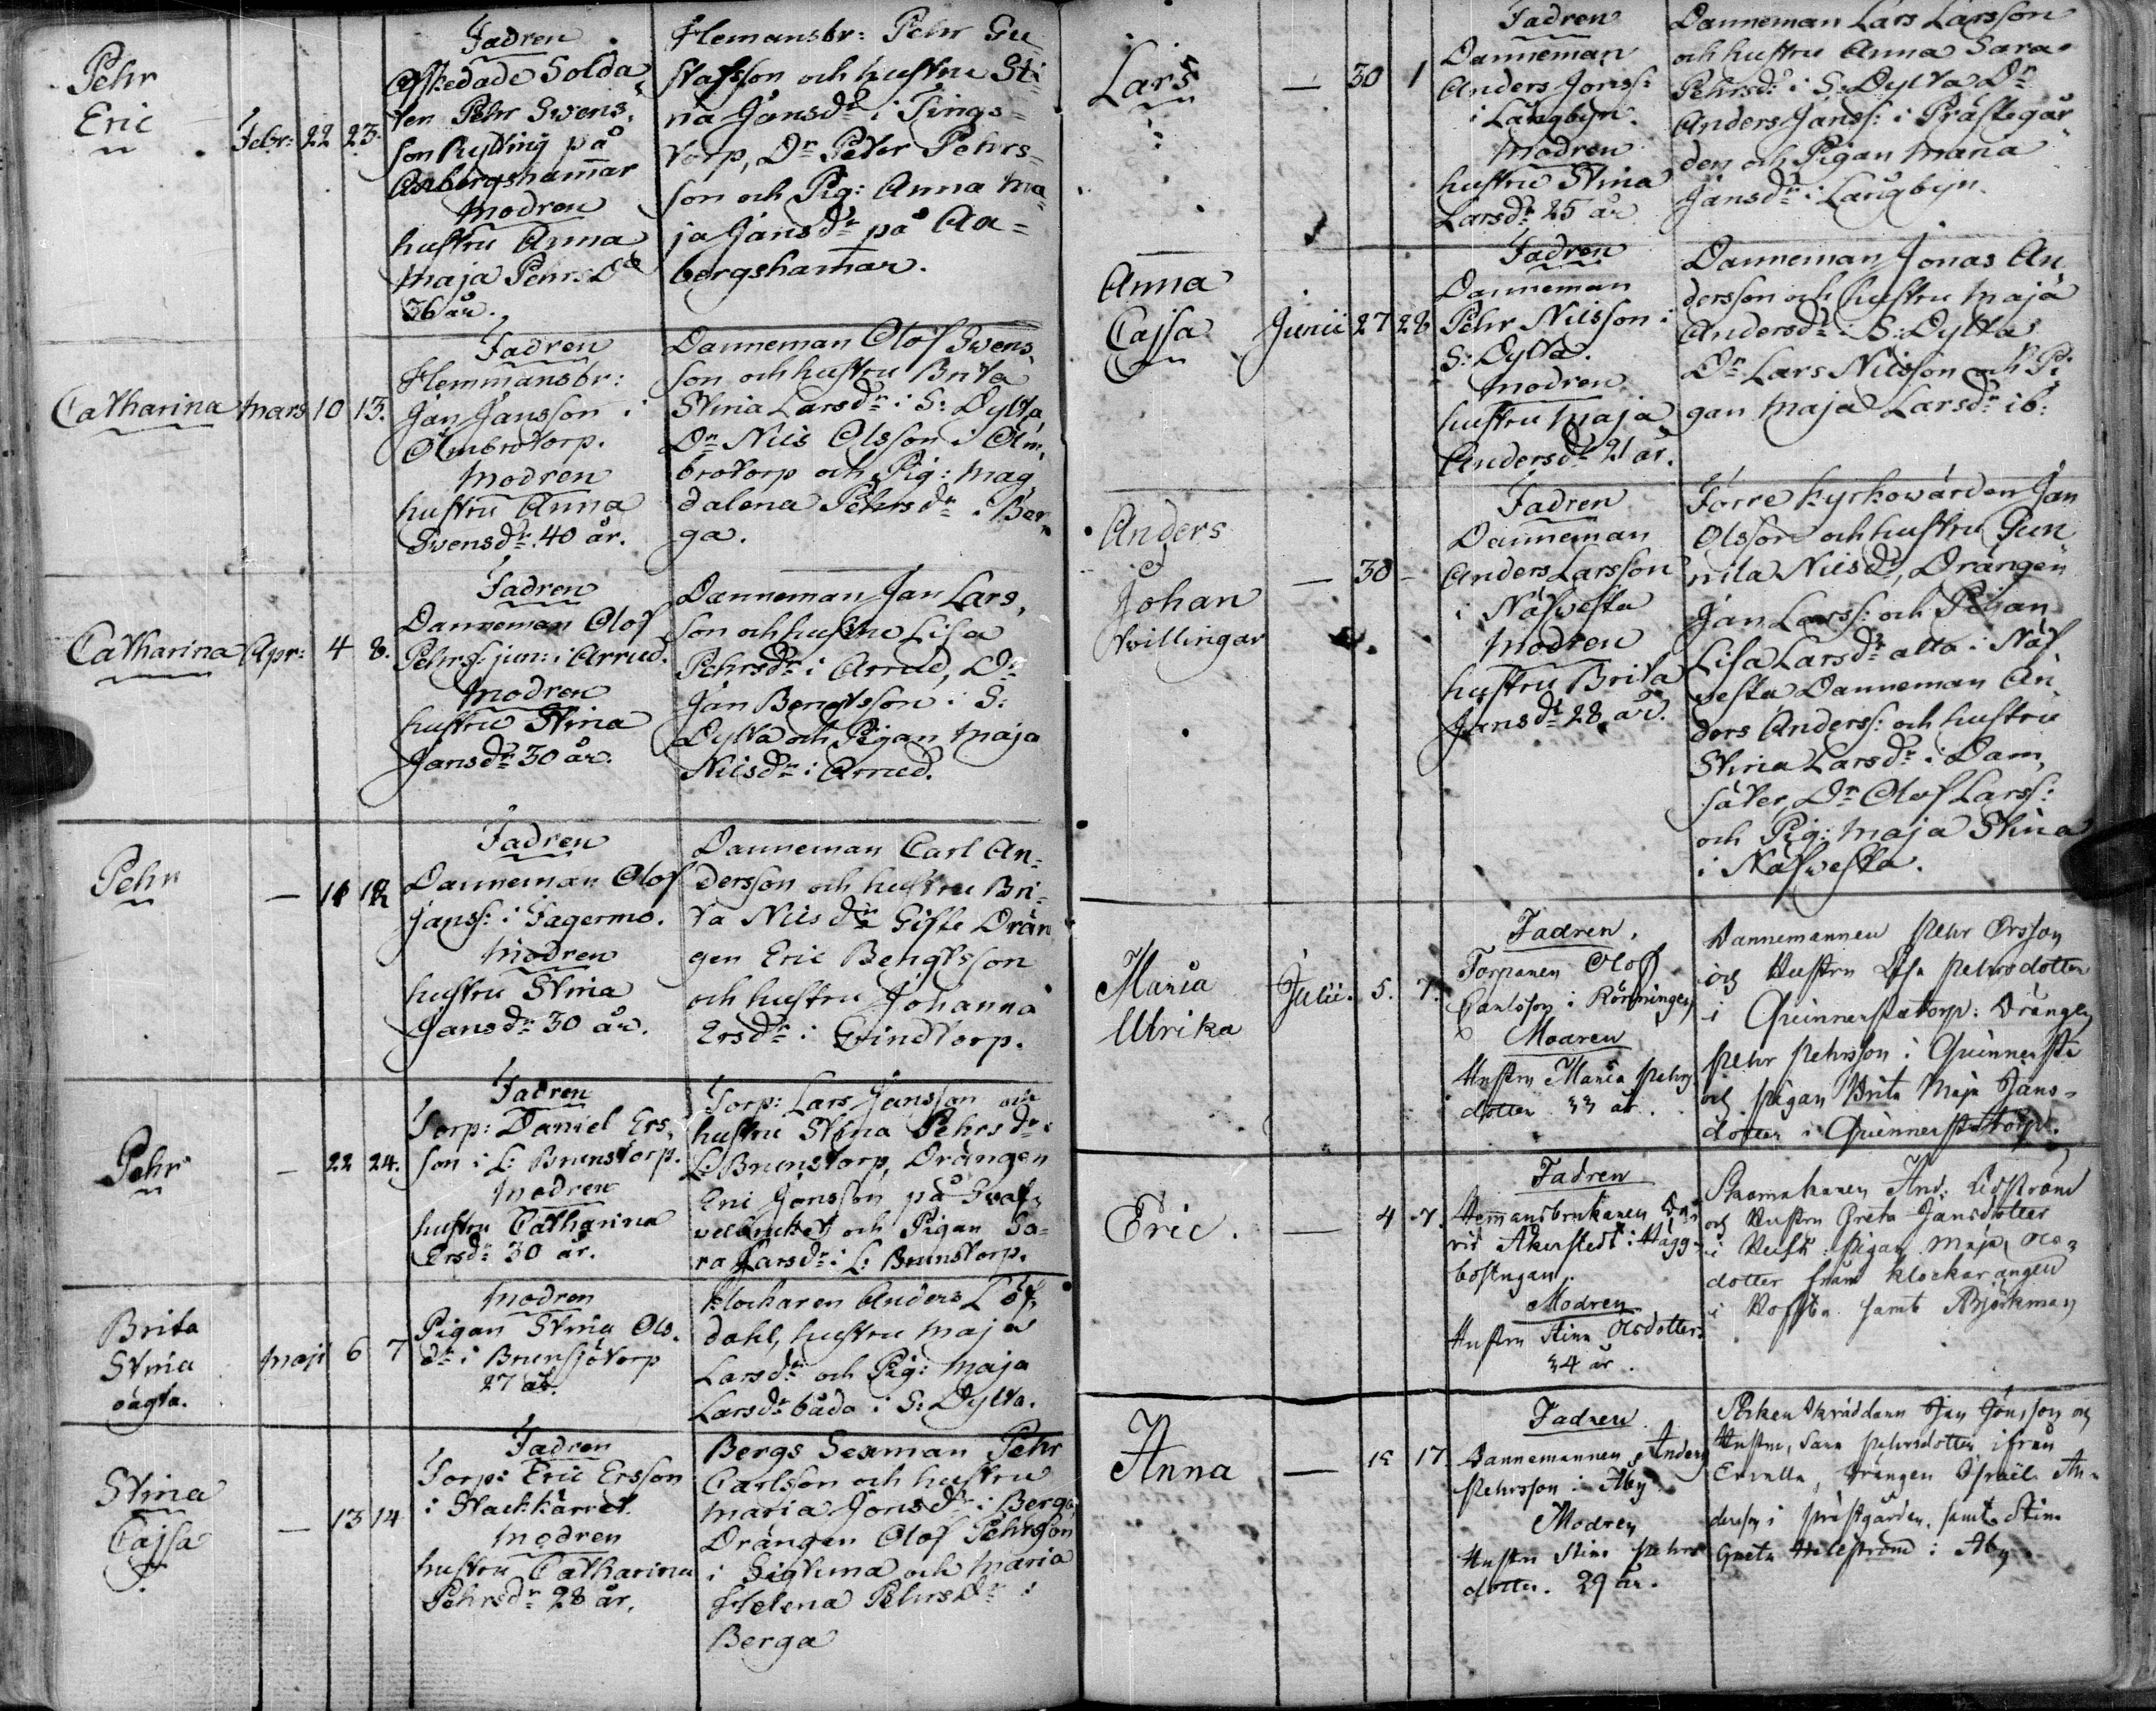
\includegraphics[scale=0.29]{resources/SWE_attention/S3HY-DRC3-H5L.jpg}
        \caption{The correct year is 1814, although the year is actually not written in the page but inferred from previous pages.}
    \end{subfigure}

    \vspace{1em}

    \begin{subfigure}[t]{0.45\textwidth}
        \centering
        
\includegraphics[scale=1.0]{resources/SWE_attention/SoftAtt/att_S3HY-DRC3-H5L.jpg}
        \caption{The base model classifies the image as 1811 by looking at the handwriting.}
    \end{subfigure} \quad %
    \begin{subfigure}[t]{0.45\textwidth}
        \centering    
\includegraphics[scale=1.0]{resources/SWE_attention/HardAtt/att_S3HY-DRC3-H5L.jpg}
        \caption{The hard attention model predicts the page as 1760.}
    \end{subfigure}

    \caption{Soft vs Hard attention on an image from the main test collection. The page comes from the book Axberg C:5 in the Örebro collection.}
    \label{fig:attention_dep_H5L}
\end{figure}


When training the Base model for one epoch with hard attention on the Swedish population records, the accuracy dropped from $8.39\%$ to $2.19\%$.
In figure \ref{fig:attention_dep_T61} we see how the soft attention partially focuses on the year and gets the prediction right while the hard attention focus on the place for the image id rather than the year.
Another example can be seen in figure \ref{fig:attention_dep_H5L} where the year is not written on the page. The soft attention guesses the correct decade by looking at the handwriting all over the page while the hard attention suggests the wrong century.

In conclusion, we see that the models with soft attention use information from all over the page to make its prediction. This includes several written years if any as well as the handwriting.
However, the single location chosen by the hard attention model does not contain enough information for making a good prediction.

Even for the simpler problem of noisy MNIST, hard attention failed because it only captured part of the digit sequence. Soft attention on the other hand could reconstruct the digit sequence by choosing multiple close locations.


\section{Post-processing} \label{sec:result_post_process}

The best result on the second dataset had an accuracy of $2.75\%$, using multi-year loss. When running the post-processing on the predictions of this model, the accuracy was increased to $3.58\%$. So even though the original predictions were quite noisy, the post-processing could still use them to boost the accuracy further.

We also tested the post-processing on the indexed part of the Örebro collection. Note that this collection was partitioned for both training and testing, so $90\%$ of the predictions are on training data. The accuracy of  Base2 was $14.9\%$ on this collection. Post-processing increased the accuracy to $15.9\%$. The mean distance between the prediction and the label was also reduced from 6 years to 4 years after post-processing.

% Works Örebro, Asker-C-2 189:
% 	 S3HT-64P3-KY5 1768 1768 [1768]
% 	 S3HT-64P3-PS4 1768 1768 [1768, 1769]
% 	 S3HT-64P3-KTG 1768 1768 [1769]
% 	 S3HT-64P3-T3Q 1771 1769 [1769]
% 	 S3HT-64P3-R81 1771 1770 [1769]
% 	 S3HT-64P3-V2C 1777 1771 [1769]

% Fail Asker-C-3 147:
% 	 S3HT-64P3-2W5 1798 1798 [1797]
% 	 S3HT-64P3-T75 1795 1798 [1797]
% 	 S3HT-64P3-NXY 1798 1798 [1797, 1798]
% 	 S3HT-64P3-233 1798 1798 [1798]
% 	 S3HT-64P3-KRW 1805 1808 [1798]
% 	 S3HT-64P3-RZP 1798 1808 [1798]

\begin{table}
\begin{subtable}{\linewidth}
\centering
\begin{tabular}{|c|c|l|}
    \hline
    Before & After & Correct \\
    \hline
    1768 & 1768 & 1768 \\
    1768 & 1768 & 1768, 1769 \\
    1768 & 1768 & 1769 \\
    1771 & \textbf{1769} & 1769 \\
    1771 & 1770 & 1769 \\
    1777 & 1771 & 1769 \\
    \hline
\end{tabular}
\caption{The post-processing can correct one of the pages to 1769. Although 1771 is not correct for the last page in the example, it is still closer to the true value than the prediction 1777.
}
\end{subtable}

\vspace{1em}

\begin{subtable}{\linewidth}
\centering
\begin{tabular}{|c|c|l|}
    \hline
    Before & After & Correct \\
    \hline
%   \textbf{h [m} & \textbf{dim [m} \\ \hline
    1798 & 1798 & 1797 \\
    1795 & 1798 & 1797 \\
    1798 & 1798 & 1797, 1798 \\
    1798 & 1798 & 1798 \\
    1805 & \textbf{1808} & 1798 \\
    1798 & 1808 & 1798 \\
    \hline
\end{tabular}
\caption{
The network makes a confident but incorrect prediction that the century digit should be 8 and the decade digit 0. The incorrect prediction makes the post-processing prefer 1808 over the true value of 1798.
}
\end{subtable}
\caption{Two examples of post-processing. In the column to the left is the prediction made by the model, the middle column contains the updated prediction after post-processing and the rightmost column contains the true label. The first example comes from the book Asker C:2 and the second from Asker C:3, both from the Örebro collection.}
\label{tab:post_process_example}
\end{table}


In table \ref{tab:post_process_example} we can see some examples of the post-processing applied to books in the Örebro collection. The post-processed sequence is typically very smooth compared to the raw predictions. Sometimes a single confident but incorrect prediction can start a long sequence of errors. One of the reasons for this is that the jump distribution strongly prefers increasing the year over decreasing the year.

\subsection{Jump distribution}


\begin{figure}
    \centering
    \begin{subfigure}[c]{1.0\textwidth}
        \centering        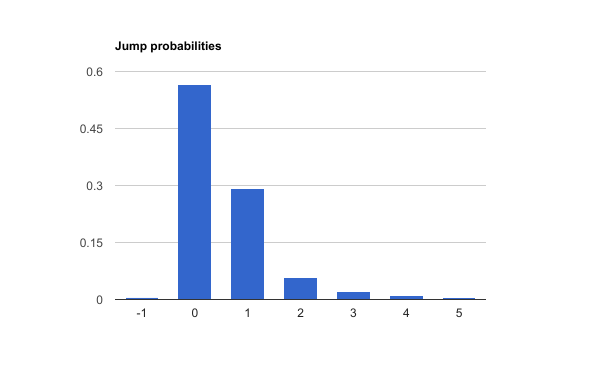
\includegraphics[scale=0.7]{resources/jump_distribution.png}
        \caption{As expected, the following page is most likely the same year or the consecutive year. With laplace smoothing of $0.5$, the probability for a zero-transition is $56.5\%$ and the probability for a plus-one-transition is $29.1\%$. The interval $[-1,5]$ contains $95.5\%$ of the smoothed distribution.}
        \label{fig:jump_prob}
    \end{subfigure}
    \begin{subfigure}[c]{1.0\textwidth}
        \centering
        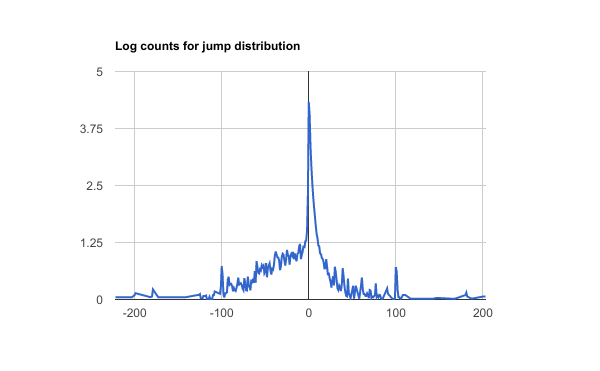
\includegraphics[scale=0.7]{resources/jump_log_counts.png}
        \caption{The plot shows $\log(1+\text{count}(x))$ for each label transition $x$.}
        \label{fig:jump_log_counts}
    \end{subfigure}
    \caption{The jump probability calculated from the training set and main test set.}
\end{figure}


The major chunk of the jump probability distribution is illustrated in figure \ref{fig:jump_prob}. We see that most page transitions should either keep the same year or increase by one.
As described earlier in section \ref{sssec:alt_postproc}, when counting transitions between two pages where both pages have multiple years, we give fractions of count to all combinations of years. This results in the small probabilities for minus one and plus two et cetera, which can be seen in the probability distribution.
% Because of multi-year labels, we also have small probabilities for minus one and plus two, since we count all combinations of .


\begin{figure}
    \centering
    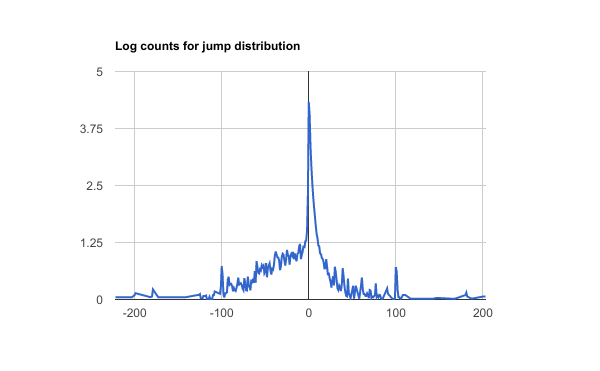
\includegraphics[scale=0.7]{resources/jump_log_counts.png}
    \caption{The plot shows $\log(1+\text{count}(x))$ for each label transition $x$ in the training set and the main test set.
    % With laplace smoothing of $0.5$, the probability for a zero transition is $56.5\%$ and the probability for a plus one transition is $29.1\%$. The interval $[-1,10]$ contains $96.3\%$ of the smoothed distribution.
    }
    \label{fig:jump_log_counts}
\end{figure}


It also happens in some books that there is a major leap between two pages as a new section of the book begins. This can be seen in the log counts for the four main collections of the Swedish population records, which is plotted in figure \ref{fig:jump_log_counts}.

\subsection{Conditional jump distribution}
One problem with the above jump distribution is that, for our dataset, a vast majority of the page transitions are zero jumps; that is from the same label to itself.
Because the distribution heavily favors the zero jump, the predictions after post-processing often output the same year for all pages in a book, instead of increasing years as we would expect.

One idea to fix this is to condition the current transition on the previous transition. The idea is that if the previous transition was a zero jump, we should be more likely to change year now. However, when aggregating the statistics for the Swedish dataset, it turns out our intuition was wrong: if the previous transition was a zero jump, it is even greater probability that the current transition is a zero jump. So a conditional distribution reinforces the problem instead of alleviating it.

\section{What have the models learned?}


\begin{figure}
    \centering
    \begin{subfigure}[c]{1.0\textwidth}
        \centering    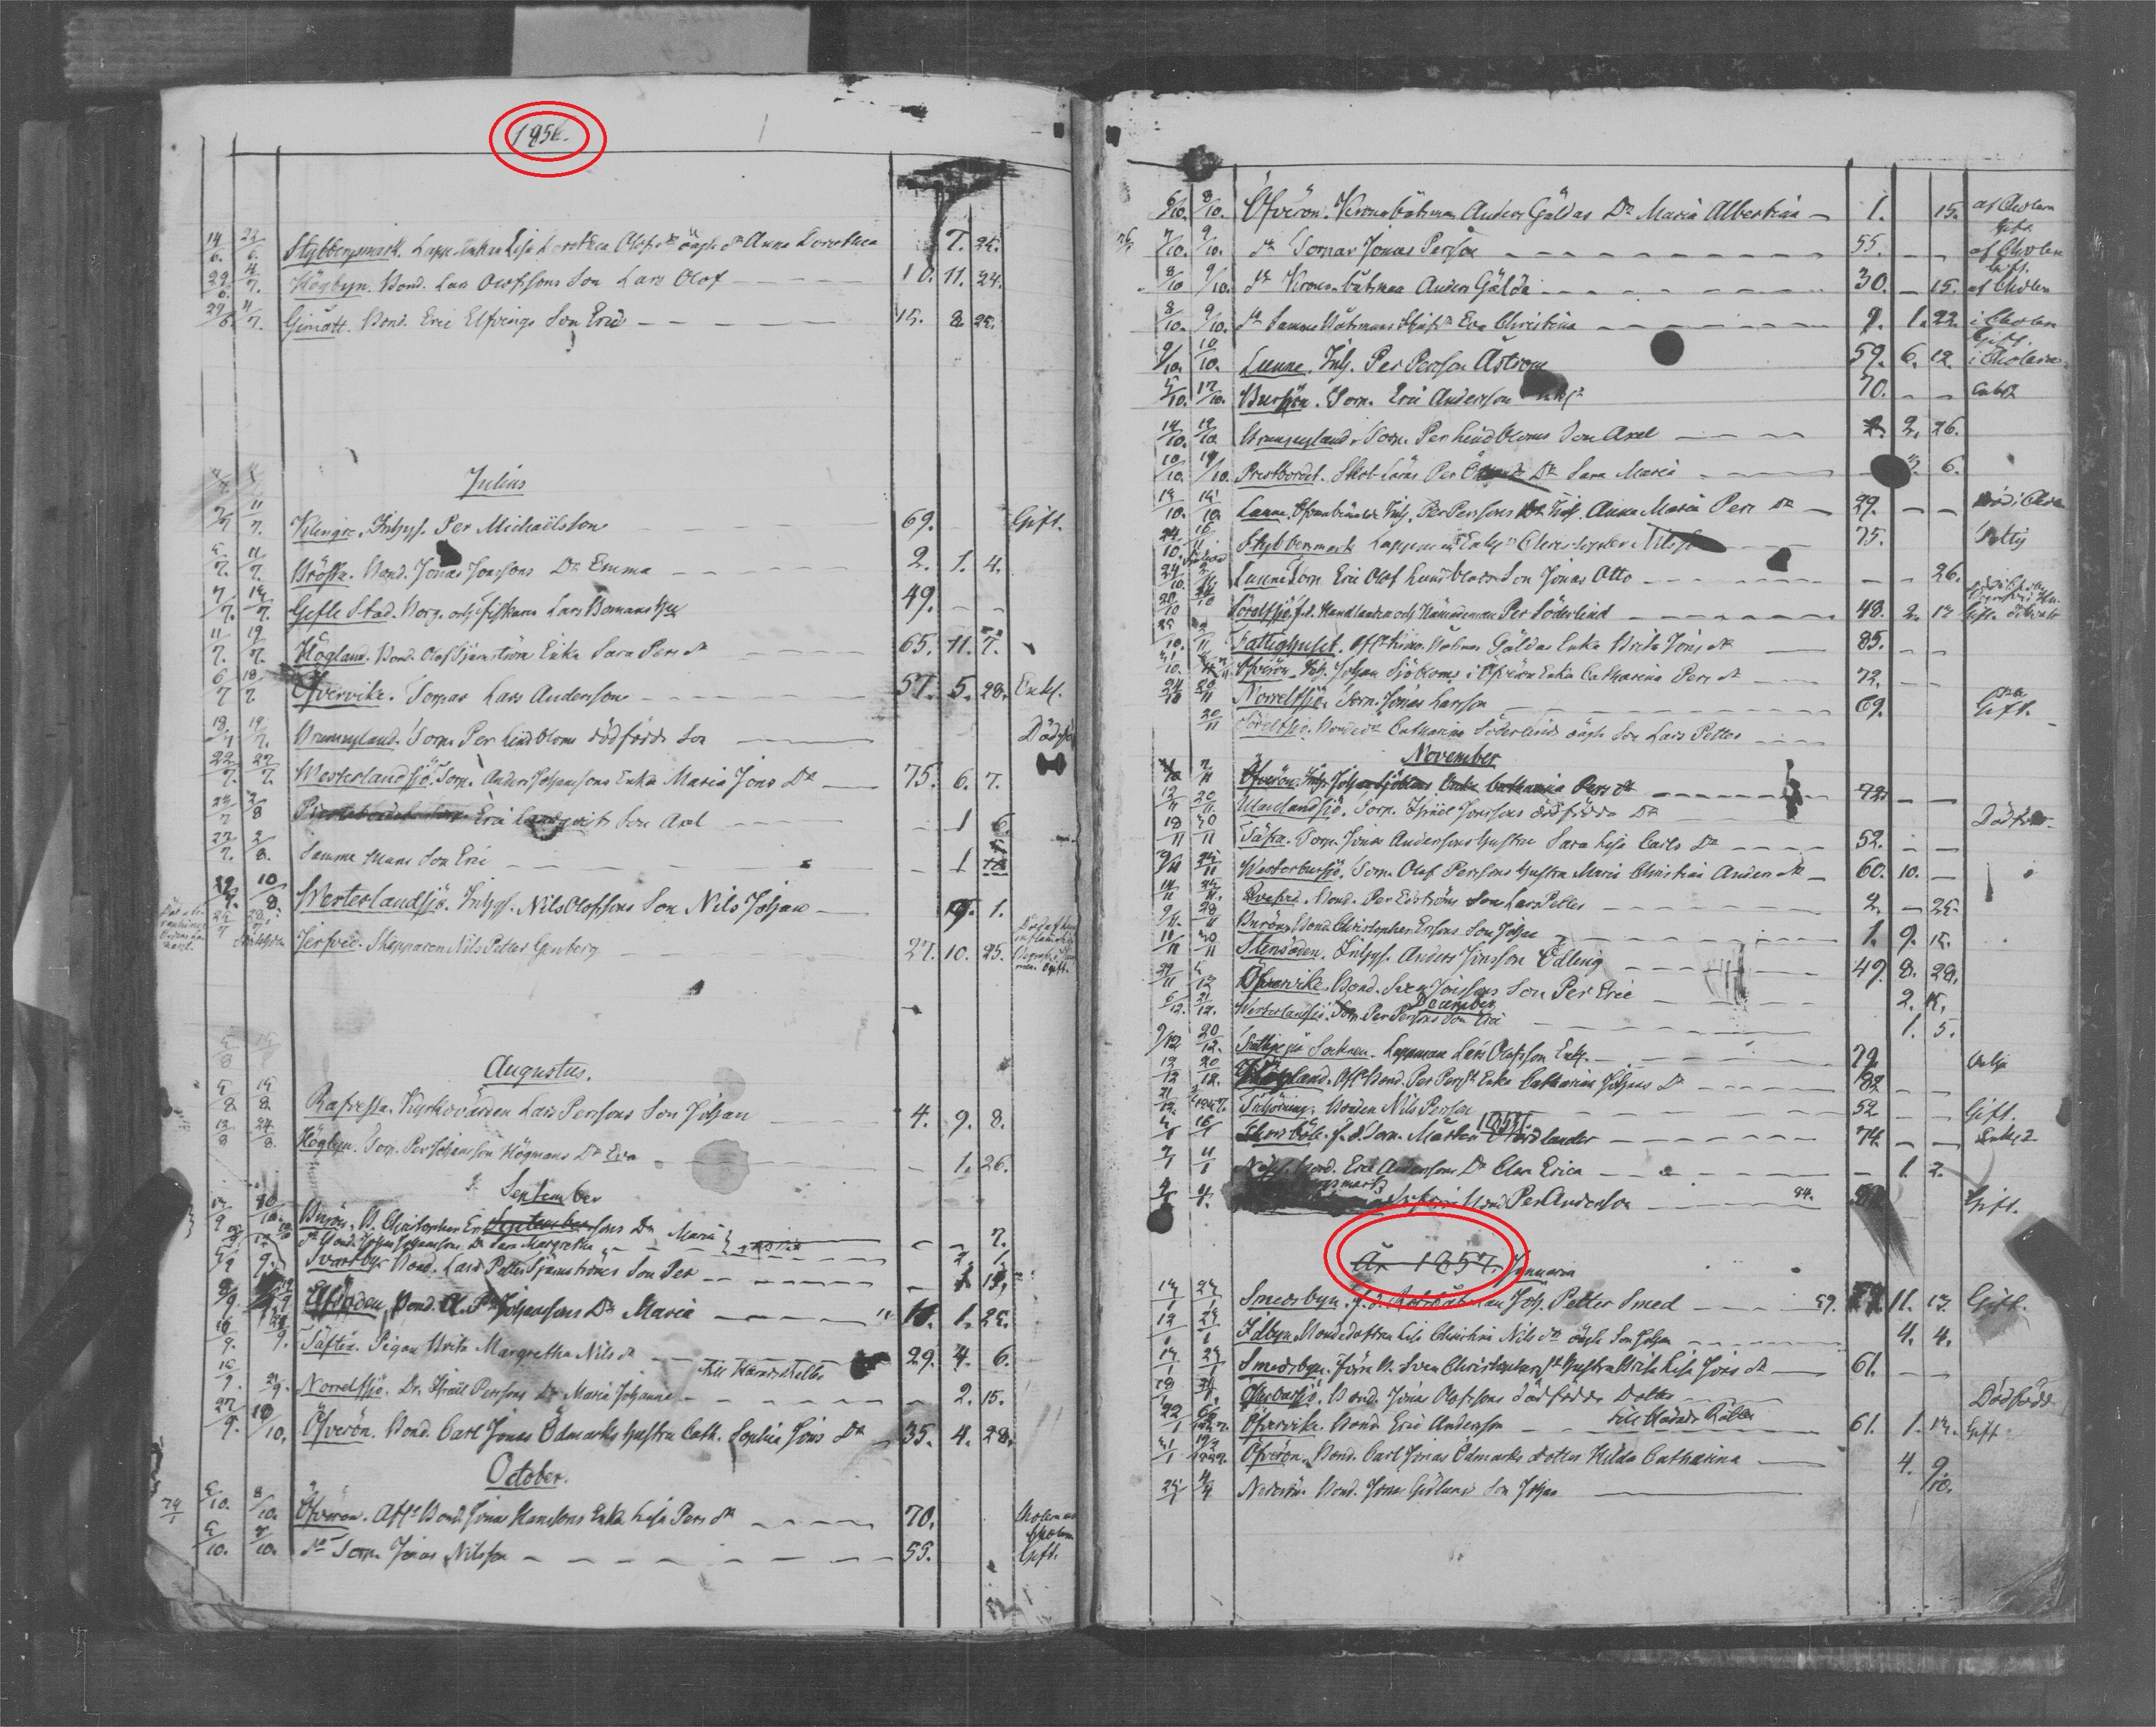
\includegraphics[scale=0.56]{resources/SWE_attention/33SQ-GRNM-9CM6.jpg}
        \caption{The correct years are 1856 and 1857, although it has been mislabeled as 1855 -- 1858 in the dataset.}
    \end{subfigure}

    \vspace{1em}

    \begin{subfigure}[t]{1.0\textwidth}
        \centering
        
\includegraphics[scale=1.0]{resources/SWE_attention/Base2/att_33SQ-GRNM-9CM6.jpg}
        \caption{The Base2 model pays attention to many of the dates along the column instead of the two written years.}
    \end{subfigure}

    \caption{The Base2 model miss-classifies this image from the second test set as 1831. The page comes from the book Arnäs C:4 in the Västernorrland collection.}
    \label{fig:attention_dep_9CM6}
\end{figure}


In figure \ref{fig:attention_dep_9CM6}, we can see that the  Base2 model learned to recognize the importance of digits, although in this particular example it payed attention to many irrelevant digits instead of the written years.

\begin{figure}
    \centering
    \begin{subfigure}[c]{1.0\textwidth}
        \centering
        % img_S3HT-64P3-2GW
        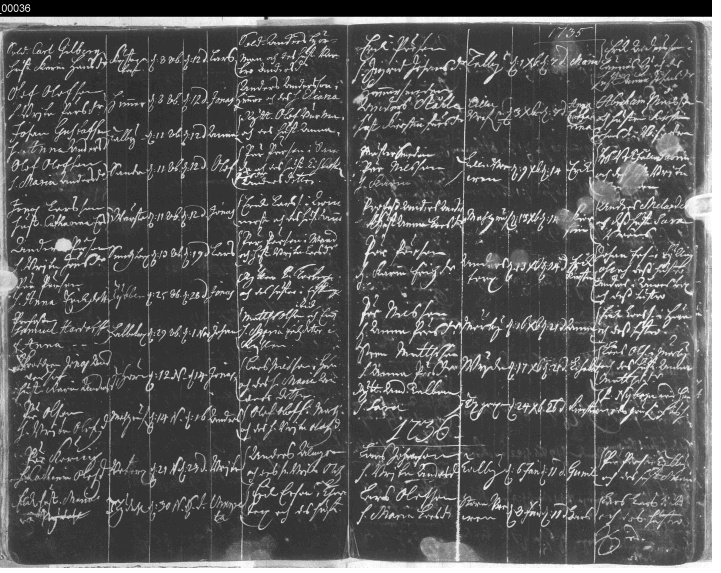
\includegraphics[scale=1.0]{resources/Edited/Orig_processed/img_S3HT-64P3-2GW.jpg}
        \caption{...}
        % \label{fig:jump_prob}
    \end{subfigure}
    \begin{subfigure}[c]{1.0\textwidth}
        \centering
        
\includegraphics{resources/Edited/Orig_att/att_S3HT-64P3-2GW.jpg}
        \caption{The ...}
        % \label{fig:jump_log_counts}
    \end{subfigure}
    \caption{Caption...}
    \label{fig:my_label}
\end{figure}

However, we hypothesized that the network had also learned to recognize other signals than digits. To test our hypothesis, we selected five images from the main test set and edited them so they no longer contained any handwritten years. The  Base2 model classified two of these five images correctly before editing. When running the model on the five edited images, the predictions were exactly the same as before editing. The attention matrix was also almost identical with and without the handwritten year. One of these five images and the corresponding attention are visualized in figure \ref{fig:edited}.

Because the network has not seen any of these five images during training, it appears to have learned to recognize the handwriting of the individual scribe who wrote the book. This is likely one of the reasons why the accuracy is so much lower for our second test set, because the model has not been trained to recognize any handwriting from that dataset.

So it seems that at least for some pages, the network makes the right prediction, not because it can read the year digits, but because it recognizes the style of the handwriting. It is not what we intended the network to learn, but it nevertheless shows the potential of deep learning that the models can even learn to recognize handwriting styles.

\newpage
\section{Summary}

We now summarize our findings and compare the different models. Table \ref{tab:model_overview} lists our models and different metrics for the two test sets.

%  & Swe_DEP_7-199 & 0.0417 & 10 & 18 & 0.262 &  &  &  &

\begin{table}
  \centering
  \begin{tabular}{|c|c||c|c|c|c||c|c|c|c|}
    \hline
    & & \multicolumn{4}{c||}{Main} & \multicolumn{4}{c|}{Secondary} \\
    % \hline
    Name & Epochs & Acc & Med & Mean & Near & Acc & Med & Mean & Near \\
    \hline
    Base & 16 & 0.0839 & 6 & 10 & 0.408 & 0.0211 & 23 & 30 & 0.113 \\
    \hline
    Ind & 16+1 & 0.0720 & 6 & 11 & 0.423 & 0.0221 & 21 & 29 & 0.129 \\
    & 16+6 & 0.0850 & 6 & 10 & 0.436 & 0.0211 & 24 & 31 & 0.111 \\
    (Base2) & 16+7 & 0.0898 & 6 & 10 & 0.429 & 0.0235 & 26 & 33 & 0.115 \\
    \hline
    Multi & 16+1 & 0.0707 & 6 & 10 & 0.400 & 0.0157 & 26 & 33 & 0.104 \\
    & 23+4 & 0.0758 & 6 & 11 & 0.410 & 0.0275 & 21 & 29 & 0.130 \\
    +post & 23+4 & & & & & \textbf{0.0358} & 18 & 28 & 0.156 \\
    \hline
    Simple & 23+1 & 0.0883 & 6 & 10 & 0.426 & 0.0216 & 25 & 31 & 0.120 \\
    & 23+6 & \textbf{0.0954} & 6 & 10 & 0.431 & 0.0142 & 26 & 32 & 0.100 \\
    \hline
    Hard & 16+1 & 0.0219 & 20 & 35 & 0.150 & 0.0152 & 32 & 41 & 0.097 \\
    \hline
  \end{tabular}
  \caption{For each model, we list for how many epochs it has been trained including pre-training, four metrics on the main test set and four metrics on the second test set for generalization.
  The first metric is accuracy, the second is median distance between prediction and correct label, the third is the mean distance and the last metric is the percentage of predictions that were less than 5 years wrong from the correct label.
  The models are the Base model, independent digit loss, multi-year loss, multi-year loss with post-processing, simplified training data and hard attention.
  Note that the models that are pre-trained with 16 epochs use the Base model, while the models that are pre-trained with 23 epochs use the Base2 model.
  }
  \label{tab:model_overview}
\end{table}


The highest accuracy on the main training set was achieved by the Simple model, which had been trained on the simplified training data without multiple year images.
Since removing the multiple years helped learning, it is clear that the multiple year labeling makes the problem more difficult.
% This illustrates how difficult the problem becomes because of the multiple year labels.
On the other hand, the same model had the lowest accuracy on the second dataset.

One possible explanation for the increased accuracy on the main test set and the decreased accuracy on the second test set is that the Simple model better learned to recognize handwriting. Since the main test set was sampled from the same books as the training set, the handwriting is the same. In contrast, the second test set does not share any scribe in common and hence has different handwriting. The fact that a model can decrease our loss function by recognizing handwriting instead of digits only testify of the difficulty of the task.

There are several possible reasons why the model would think that the background text is more predictive of the year than the digits. Firstly, there are many other digits in the images than years and we give no credit for recognizing other digit sequences, such as dates. Secondly, the year digits are written by so different handwriting styles that it may be difficult to distinguish the year from the text, which is also very varied. After all, most signals for digits would also trigger for some letters.
Thirdly, the handwriting style may actually differ so much between books and time periods that it is predictive of the decade, or at least the century.

However, for the system to be useful, it should generalize well to new collections, such as the second test set. The model with highest accuracy on the second test set was using multi-year loss and the accuracy could be boosted further by using our method for post-processing.
Since this model used a new loss function, it is possible that the increased accuracy simply came from reduced overfitting. To know for sure, we would need to retrain the model from scratch, which would take some weeks.

Although we were not able to predict the exact year with high accuracy,
many of our models could guess the correct decade in the main test set with more than $40\%$ accuracy. One can argue that the model could recognize the approximate time by recognizing the page structure of individual books. However, since the attention model only accesses small locations in the image at a time and the decoder sums over said small locations, it seems somewhat unlikely that the network would recognize page structures. On the other hand, local features like vertical column lines could constitute a learned indicator for certain books.

Although hard attention did not work very well for us, if the network could successfully identify the places of the year, hard attention would work quite well. One way to achieve this would be to add a separate loss for the attention model based on bounding boxes in the training data. Hard attention would in that case make sure that we actually would predict based on the year digits and not on the handwriting style. However, at the moment, there are no such bounding boxes for the Swedish population records.

% TODO check page


\chapter{Alternative methods}
% "conventional methods" ?
\textit{ We have previously described how neural networks, especially convolutional neural networks, can be applied to image classification problem, and by extension, transcription.
For completeness, we here give a brief overview of some alternative methods for handwriting recognition and transcription that are not used in this thesis.
In the next chapter we compare our work with previously mentioned related work and consider segmentation for future work, which is introduced in this chapter.
}

% In this section we describe traditional methods for related tasks: text recognition and word spotting. In this thesis however, we have chosen to use a different approach based on neural networks, which are discussed in depth in section \ref{sec:networks}.

%% Rewrite this part, add more recent work, especially in deep learning and CNNs: spatial transformations, visual-semantic alignment etc.

\section{Handwritten text recognition} \label{sec:alt_htr}

\textbf{Handwritten text recognition} (HTR) systems have
% been employed successfully in industry for
seen commercial success in
% been employed with commercial success for
recognizing postal addresses on letters \cite{lecun_1989, zipcode_system} and reading bank cheques. This has been possible because (1) the text is in a very small domain and (2) these applications have high market value \cite{40_years_HWR}. However, transcribing a natural language in general is still an unsolved problem.

% \subsubsection{}
HTR solutions can typically be described by four steps \cite{offline_HWR_CNN}:
\begin{enumerate}
    \item Pre-processing - each pixel in the image is mapped to either 0 or 1, skew is corrected and noise is removed.
    \item Segmentation - the image is cut into small segments, so that each segment contains a handwritten word.
    \item Feature extraction - each image segment is encoded into some vector of features.
    \item Classification - the feature vector is interpreted as a word from a known vocabulary.
\end{enumerate}

A comprehensible survey of common techniques for the different steps can be found here \cite{HWR_survey}.
Previous work on HTR include \textbf{Hidden markov models} (HMMs) in combination with neural networks \cite{Offline_HWR_HMM_ANN}.
More recent approaches include multi-stream HMMs \cite{HWR_multi_stream_HMM_arabic}, HMMs with \textbf{recurrent neural networks} (RNNs) \cite{Offline_HWR_RNN} and deep \textbf{convolutional neural networks} (CNNs) \cite{offline_HWR_CNN}.

\subsection{Pre-processing}

Pre-processing is commonly used to improve the quality of the input \cite{HWR_survey}. However, successful attempts have been made without pre-processing \cite{FornesCnnCategorization}. We only describe binarization and skew detection but \textbf{noise reduction} and \textbf{line detection} are also common pre-processing tasks.

\subsubsection{Binarization}

Binarization maps each pixel to 0 or 1 depending on whether the gray-scale value of the pixel is above or below some threshold.
Binarizing the image is necessary for some techniques that count black pixels
% such as projection-based skew detection,
or use connected components (CCs). A connected component is simply a group of adjacent black pixels surrounded by white pixels in the binarized image.

The simplest is to use a global threshold, often calculated by Otsu's method. Otsu's method looks at the intensity histogram of the image. Assuming that there are two peaks in the histogram, one for background and one for foreground, it attempts to find a balanced threshold between the peaks. If the lighting was uneven at the time of photography, global thresholding does not work very well.

Another approach is to use local or adaptive thresholds, which calculates different thresholds for each pixel depending on the surrounding area. Local thresholds are more successful than global thresholding on low quality images, especially in the presence of noise. There are extensions to Otsu's method to produce local thresholds.

Neural networks have also been used to combine global and local thresholds for binarization.

\subsubsection{Skew detection}

Skew, or rotation, in images of text can be detected by computing the horizontal projection for different angles. The horizontal projection counts the number of black pixels per row, which requires the above described binarization. The amplitude of the projection is maximized when the image rotation is aligned with the text.

% \subsubsection{Noise reduction}
%
% Median filtering...
%
% \subsubsection{Line detection}

\subsection{Segmentation}

Segmentation produces bounding boxes around detected words in the input image to be transcribed. The resulting word images can then be used as input for feature extraction. In order to produce word segments, most methods first segment the text lines.

There are many methods that have been proposed for word image segmentation \cite{HWR_survey, Waterflow2011, Waterflow2015}.

\subsubsection{Projections}

The simplest group of methods is based on projections of the image. For example pixel counting, which cuts the image into line segments on the rows where the number of black pixels is below a threshold. However, this approach assumes the text to be written on straight lines, which is often true for printed text but it does not hold for free-form handwriting. Another problem is if there are multiple lines in the image which are not aligned.

\subsubsection{Smearing}

Smearing is another group of methods that grows a boundary from each black pixel and groups the black pixels whose boundaries overlap. The water flow algorithm seems promising from this group of methods since it can handle curved text quite well \cite{Waterflow2011, Waterflow2015}.

\subsubsection{Graphs}

Another successful approach is to represent the connected components in the binarized image as vertices in a weighted graph \cite{GraphSegmentation}.
% For each pair of connected components we compute a connectivity metric $c$, which is based on the Euclidian distance, and form an edge between the corresponding vertices with weight $c$.
For each pair of vertices we create an edge, whose weight takes the value of a connectivity metric based on the Euclidian distance between the two connected components.
% We compute a connectivity metric based on the Euclidian distance between all connected components.
% Each edge between two vertices takes a weight
% For weights, we use a connectivity metric that is based on the closest Euclidian distance between the two connected components.
% The weight between two vertices is based
% Every edge between two vertices is associated with a connectivity metric,
% The edges of the graph use a connectivity metric for weight,
% which is based on the closest Euclidian distance between the two connected components.
% The minimum spanning tree for the graph can be computed and cut into subgraphs which become segments. The cutting can be done by using a pre-determined threshold for the connectivity metric.
The segments are created by cutting the minimum spanning tree of the graph at every edge whose weight is lower than some pre-determined threshold.

\subsubsection{Recursive}

Yet another approach is recursive methods, which use a reference library of word images.
Recursive methods attempt to find a sequence of segments such that each segment matches some reference word image within a pre-defined error threshold.
% attempt to find a sequence of segments so that each segment matches some word image within a certain error threshold.
One obvious problem is that the method requires a library that contains similar words as in the image. On the one hand, genealogical records use the same words many times like \textquote{born} and \textquote{father}; on the other hand, handwriting has so many variations that it may be difficult to create a sufficiently large library.
% Since handwriting has so many variations, it may be difficult to create a sufficiently large library.



% Stochastic methods utilize HMMs to ...



% \section{Word spotting}
%
% Mention alternative approach to aid waypointing by using segmentation free word spotting to compile word image clouds. However, does not help towards automated indexing. Cite Uppsala.
%
% \section{Named entity recognition}
%
% \textbf{Named entity recognition} (NER) ...?

\chapter{Conclusion}

\textit{In this chapter we compare our results to previous work and suggest future research for solving the problem of automated indexing.}

% \section{Things we would have done differently}
% \textbf{TODO}: change title of section
%
% Encoder should also be trained using dropout as \textcite{multidigit_streetview}.
%
% Retrain network from start for each experiment, however takes too much time.


\section{Our work compared to previous work}

For only helping waypointing, we could produce image-based word clouds to summarize books as performed on historical documents by \textcite{ImageCloud}. Another possible approach for alleviating waypointing would be to use word spotting, which allows searching over images for either a query string or a query image \cite{WordSpotting}.
In this thesis, however we want to find the relevant information from every page and we want to output transcribed text instead of images. Applying word spotting by query string on separately on every page would work in theory but this requires a dataset of transcribed word images for training which we do not have.

One of the challenges in classifying year for a page is the sheer size of the page. Downsampling reduces the size of the image but also makes recognition more difficult as the resolution decreases. Large images take a long time to process and they may also contain much unrelated information. When recognizing house numbers from Google Street View, \textcite{multidigit_streetview} first made an automated system that cropped out the part of the image containing house numbers as a fixed size $128 \times 128$ region, which was then fed to their CNN for classification. In our thesis, the attention model would be the corresponding mechanism for choosing a subregion in the image. However, the attention model requires the encoder CNN to run on the entire image, which increases running time.
One benefit of using an attention model is that the system is trainable from end-to-end.
However, as we have seen in our results, the attention model does not always learn to focus on the things we intend it to.

\textcite{FornesCnnCategorization}, who worked on automatic transcription of civil population records, also ran their models on small word images compared to the entire pages. In this case, they made no automatic system for segmenting the images but manually created a small dataset of word images with corresponding transcriptions \cite{esposalles}.

In contrast, for the task of image captioning, both \textcite{AttendAndTell} and \textcite{VisualSemanticAlignment} run their CNNs directly on large images. Both use some kind of alignment model, R-CNN or attention, for associating labels without location to some part of the image.

However, \textcite{AttendAndTell} use a model pre-trained on ImageNet, which contains millions of labeled images. This means that their encoder was already good at recognizing various animals and objects necessary for generating a descriptive caption. \textcite{VisualSemanticAlignment} on the other hand employ a hard-coded algorithm for finding regions that are most probable to contain an object of interest, which in handwriting recognition most closely would correspond to segmentation.
In our work, we pre-trained our model on the noisy MNIST, but it appears that the handwriting in MNIST is too different compared to Swedish handwriting during the 18th and 19th century to make any significant impact.

Another difficulty we face is that in order to correctly classify a year, the model must pay attention to all digits in the year. However, in object recognition and image captioning, focusing on a leg might still be sufficient to recognize a cate.

Furthermore, the model of \textcite{AttendAndTell} revisits the image in each iteration as it generates new words for the caption. The hidden state of the decoder is fed as auxiliary input, so that the attention model will focus on new parts of the image. Thus, if the model would focus on the wrong thing to start with, it can still remedy the situation in later iterations.
In our model, we only generate a single year so we only allow the model to look once at each image. Although it is conceivable to make a recurrent decoder for our task, it would significantly complicate the model.

% In conclusion, our task is very difficult since the images are large and they contain much unrelated information which look very similar to the relevant signals.

% Compared to our task, there are however some major differences.
% Firstly, image captioning do not transcribe information in the image but generate a descriptive text, which typically involves recognizing objects in the image.
% their model was pretrained on ImageNet, which contains several million images.

% In contrast, \textcite{AttendAndTell} run on the entire input image while using attention to find the elements of interest. However, they do not transcribe any text but rather recognize objects in the image in order to generate new text. Hard attention, where the decoder only uses a single output unit from the encoder, worked rather well for object recognition but not so well for transcription. We conclude that a decoder can recognize objects without seeing them entirely, for example a leg might be enough to recognize a cat but a decoder can not guess the correct sequence of digits if it can only see the first two digits out of four.
% A key difference is that one output unit can recognize as an object without seeing it entirely, a piece of fur can be enough to recognize a cat while for transcription we need the network to consider the entire sequence.

% Another major difference between our work and \cite{AttendAndTell} is that their decoder was sequential so for each iteration it looked at a new part of the image. So even though the decoder only looked at a single place in each iteration, over the output sequence most relevant parts of the image had been covered.

% Difference: our attention model has no hidden state as auxiliary input. However, should not need one since always want to see year and nothing else.

\section{Future work}

From our findings, it seems that attention mechanisms after running on the entire image is less suitable for information extraction and transcription than for object recognition and caption generation. In our training, we did not see any overfitting yet so there may be more potential for these methods by training longer and on better hardware.

Another future approach could be to incorporate spatial transformer modules in the network, as presented by \textcite{SpatialTransformerNetworks}.
However, running on entire input images with only loose labels is slow and the model learns to recognize other features than intended, since the background text is too difficult to distinguish from the years and too seemingly predictive to ignore.
Instead, it seems that the conventional approach of segmenting the page image to word images is the best way to go. However, there are two major challenges with segmentation.

Firstly, the words have to be segmented correctly. This has proven to be a challenging problem in itself and much research has been spent on finding good methods of segmenting handwritten text. For evaluating the segmentation methods, the Esposalles dataset \cite{esposalles} can prove very useful since it contains bounding boxes of word images in civil population records.

Secondly, the segmented images would need to be associated with the labels, either manually in the dataset as by \textcite{esposalles} or latently during training.
\textcite{VisualSemanticAlignment} successfully found alignment between weak labels and explicit regions in their dataset. However, as we have seen in this thesis, latently associating the label with a region in the input may lead to unexpected results. On the other hand, manually segmenting and transcribing hundreds of thousands of images of population records is a daunting task.
 % Perhaps this can be done latently as by \textcite{VisualSemanticAlignment} or manually as by \textcite{esposalles}.

For the purpose of making a fully automated indexing system, there are two major approaches to consider. Either one can make a model that exactly transcribes the word images as \textcite{FornesCnnCategorization} and then follow up by a language model, or a model that attempts to directly extract the genealogical information from the word images. The latter may prove difficult as some word images need to be ignored and other information depends on previous words. For example, to correctly extract a birth date, the model would need to remember the month which may have been written several records above.
A benefit of an extraction model is that it would be trainable from end-to-end. However, it is unclear what would be a suitable loss-function for such a task.

The other approach would however require two datasets that we do not have. An exact transcription system would need to train on word images with corresponding transcriptions, like the Esposalles dataset \cite{esposalles}. However, creating such a dataset of sufficient size seems infeasible considering the great variation in spelling and handwriting for genealogical documents. We also observe that the Esposalles dataset was originally intended to grow to cover more books, but after several years it is covers only a few pages. The second training set would require a language model that would take the transcriptions as input, understand the relations and then generate the indexed information. Again, training such a language model would require a corresponding dataset in all relevant languages from various centuries, which we do not have.

In conclusion, the most feasible approach for making a fully automated indexing system seems to be to train a model for segmentation on the Esposalles dataset \cite{esposalles} and then make an end-to-end system for information extraction that would use the indexed information directly as labels. Although this is a difficult task, it seems more feasible than manually creating the necessary datasets for exact transcription and language modeling.

For future information extraction systems that would attempt to latently associating indexed information with word images, this thesis provides a baseline on the Swedish population records dataset for extracting the main years.

% On the other hand, given the scope of our long-term goal, it is infeasible to produce a sufficiently large dataset for training a model that exactly transcribes each word.

% On the other hand, a model for extract transcription seems unprobable as it would require considerable

% On the other hand, a model for exact transcription would require a much more detailed dataset than we have available and

% Secondly, it is not clear how the transcription or extraction model could be trained using the indexed data. The primary problem lies in how to associate the extracted information with the segmented word images. It would likely take much manual work to create a trainable dataset, but there are two approaches to this. 1. The entire text could be transcribed exactly as in the case of \cite{esposalles}. Doing so would be useful if the final system has separate models for transcription and named entity recognition.
% 2. Each piece of extracted information could be associated with a word image. That would mean that some word images have no label and should be ignored although they may actually contain information.

% Whichever approach is taken between exact transcription followed by language model and direct information extraction, the end-to-end system must learn which information is relevant and which is not.
% For indexing purposes, we are only interested in the date, location, person, age and close relatives. Ignored information include baptism witnesses and summaries of life stories upon death.
% For example, baptism witnesses consist of many names but not much useful information for genealogical research.

% Since the indexed data is not a transcription of text but rather extracted information, several word images could contribute to a single piece of information.



%------------------------------

%\newpage
%\addcontentsline{toc}{section}{References}

\cleardoublepage
% \addcontentsline{toc}{chapter}{Bibliography}
\printbibliography


\newpage

% \begin{appendix}
% 
\section{Genealogy}

Genealogy is the study of one's ancestors. It involves finding who they were, the time and place of their birth, where they lived, how their life was, how their life eventually ended and how their family continued to present day.

Getting to know and comprehend the lives of one's ancestors can have great personal significance as one can feel more connected with people in centuries past. One can gain appreciation for parents and forefathers and their efforts so that oneself could be born.
Experiences can also be learned from important events, stories and hardships in the lives of one's ancestors and one can more easily appreciate how many things are different today, although as human beings we are perhaps not so different.

Many people are familiar with the lives of their parents and perhaps also the their grandparents from just listening to them.
However, each generation further back requires more study and effort to explore as the records get more sparse, get harder to access, are written in an older language and in a handwriting style that get increasingly different from the handwriting of today. Furthermore, because each child has two biological parents, the number of ancestors increases at least by a factor of two in each generation.

The advance of technology has been very instrumental in making the genealogical research easier and more accessible. Instead of traveling to different vaults of the records, people could order microfilms with photographs to view at home or at a nearby genealogy center. With the Internet, people can currently access many records directly online as images. A future big leap forward consists of the indexing effort which makes it possible for people to search the records with search engines and databases instead of manually scanning through and reading the pages.

Manually indexing a book from cover to cover has a very high throughput of data compared to searching the pages for a single entry because 1. it takes time to get accustomed to the handwriting of that particular scribe as well as locations in that parish 2. the time for each entry is significantly reduced as one does not need to search through many pages. So although it is not viable for a single person to do, if many people contribute, it lowers the total workload in the end for the community.

However, indexing takes a lot of effort and also some experience in reading old handwriting. If computers could index the records themselves with only minor human contribution, that would significantly improve the indexing rate and hence produce a very powerful tool for the entire genealogical community.

Solving waypointing is not as significant as indexing but would constitute a stepping stone towards indexing in extracting information from the records in an automated manner.
% as well as reducing manual labor for waypointing.
Waypointing in itself is also useful as more images can be published online under the correct categories. Automating waypointing would free time in favor of genealogical research and indexing.

% \end{appendix}


\end{document}
